\documentclass{article}
\usepackage[utf8]{inputenc}
\usepackage{amsmath}
\usepackage{amssymb}
\usepackage{graphicx}
\usepackage{tabularx}
\usepackage{booktabs}
\usepackage[english]{babel}
\usepackage{setspace}
\usepackage{geometry}
\usepackage{float}
\usepackage{url}
\usepackage{listings}
\usepackage{xcolor}
\usepackage{longtable}
\usepackage{multirow}
\usepackage{adjustbox}
\usepackage{array}
\newcolumntype{Y}{>{\raggedright\arraybackslash}X}
\newcolumntype{P}[1]{>{\raggedright\arraybackslash}p{#1}}
\usepackage{tikz}
\usetikzlibrary{positioning, calc, arrows.meta}
\usepackage[justification=centering]{caption}

\lstset{
    basicstyle=\ttfamily\small,
    backgroundcolor=\color{gray!10},
    frame=single,
    breaklines=true,
    columns=fullflexible
}

% APA style formatting
\geometry{a4paper, margin=1in}
\setstretch{1.5}
\setlength{\emergencystretch}{3em}
\captionsetup[table]{labelfont=bf, justification=centering, singlelinecheck=false}
\captionsetup[longtable]{labelfont=bf, justification=centering, singlelinecheck=false}
\captionsetup[figure]{font=small, labelfont=bf, justification=centering, singlelinecheck=false}

% Notation helpers
\newcommand{\R}{\mathbb{R}}
\newcommand{\slog}{\operatorname{slog}}
\newcommand{\ind}{\mathbf{1}}
\newcommand{\E}{\mathbb{E}}

\title{Machine Learning for Customer Churn Prediction\\[0.3em]\large Workshop 5: Generative Adversarial Networks for Synthetic Customer Sequences}
\author{Nelson David Posso Suarez \\ Javier Alejandro Penagos Hernandez \\ Nicolas Castro Rivera }
\date{}

\begin{document}

\maketitle

% ─────────────────────────────────────────────
\section{Problem Statement}
% ─────────────────────────────────────────────

In this workshop we train generative adversarial networks (GANs) to produce synthetic KKBox customers. We start from the data already prepared in Workshop~2: each manual payer is a sequence of 90 consecutive days with 14 channels per day, 8 for listening and 6 for payments (Table~\ref{tab:w5_channels}). A synthetic customer is a new $90 \times 14$ matrix in exactly that format, so it can be fed to the Workshop~2 models without any change.

We use two GAN architectures for sequences. The first is TimeGAN \cite{yoon2019}, trained with the binary cross-entropy loss of the original GAN, which is our vanilla baseline. The second replaces its adversarial loss with the Wasserstein distance and a gradient penalty (WGAN-GP) \cite{gulrajani2017}; we call it the Wasserstein TimeGAN. The work follows the five goals of the workshop:
\begin{enumerate}
    \item \textbf{Vanilla GAN.} Train TimeGAN, generate synthetic customers and inspect them visually (Sections~\ref{sec:w5_timegan} and~\ref{sec:w5_quality}).
    \item \textbf{Stable training with WGAN-GP.} Implement the Wasserstein TimeGAN and compare its convergence and generation quality with TimeGAN (Sections~\ref{sec:w5_wgan} and~\ref{sec:w5_training}).
    \item \textbf{Generation quality.} Measure realism with a Fréchet distance computed on the features of the Workshop~2 classifier, discriminative and predictive scores, marginals and domain checks, and assess it qualitatively (Section~\ref{sec:w5_quality}).
    \item \textbf{Failure modes.} Diagnose mode collapse, the discriminator overpowering the generator and the cost of the first Wasserstein implementation (Section~\ref{sec:w5_failures}).
    \item \textbf{Data augmentation.} Retrain the Workshop~2 models on real plus synthetic data and on synthetic data only, and compare them with the baseline trained on real data (Section~\ref{sec:w5_augmentation}).
\end{enumerate}

The code is in \path{workshops/w5/}: the networks in \path{models/}, the metrics and figures in \path{evaluation/}, and two notebooks. \path{w5_gan_models.ipynb} trains and evaluates TimeGAN and the first Wasserstein TimeGAN; \path{w5_wgan_tcn.ipynb} explains why that first version was replaced and evaluates the final one.

% ─────────────────────────────────────────────
\section{Data}
\label{sec:w5_data}
% ─────────────────────────────────────────────

\subsection{Input Tensor}

The GANs read the calendar tensor of Workshop~2 (\texttt{export-sequential-v6-manual}), built from the KKBox churn dataset \cite{kkbox2017}: manual payers of the February cohort, whose 90-day window ends on 2017-01-31, with churn measured in February. Day 0 is the oldest day and day 89 the cutoff. Table~\ref{tab:w5_channels} repeats the channel definition. Listening channels are zero on days without a log row; payment events are written only on payment days; payment states are carried forward from the last payment until the next one changes them.

\renewcommand{\arraystretch}{1.3}
\begin{longtable}{|c|l|c|p{6.4cm}|l|}
\hline
\textbf{Index} & \textbf{Channel} & \textbf{Group} & \textbf{Description} & \textbf{Encoding} \\ \hline
\endfirsthead
\hline
\textbf{Index} & \textbf{Channel} & \textbf{Group} & \textbf{Description} & \textbf{Encoding} \\ \hline
\endhead
\hline
\multicolumn{5}{r}{\small\textit{Continued on next page}} \\
\endfoot
\hline
\caption{The 14 channels of the Workshop~2 tensor, generated by the GANs.}
\label{tab:w5_channels}
\endlastfoot
0  & num\_25              & Listening & Songs played less than 25\% & $\log(1+x)$ \\ \hline
1  & num\_50              & Listening & Songs played 25 to 50\%     & $\log(1+x)$ \\ \hline
2  & num\_75              & Listening & Songs played 50 to 75\%     & $\log(1+x)$ \\ \hline
3  & num\_985             & Listening & Songs played 75 to 98.5\%   & $\log(1+x)$ \\ \hline
4  & num\_100             & Listening & Songs played at least 98.5\% & $\log(1+x)$ \\ \hline
5  & num\_unq             & Listening & Unique songs played         & $\log(1+x)$ \\ \hline
6  & total\_secs          & Listening & Seconds listened            & $\log(1+x)$ \\ \hline
7  & active               & Listening & 1 if a log row exists for the day, 0 otherwise & flag \\ \hline
8  & tx\_count            & Event & Number of payments on the day & $\log(1+x)$ \\ \hline
9  & tx\_paid\_sum        & Event & Total amount paid on the day (NTD) & $\slog(x)$ \\ \hline
10 & tx\_plan\_days\_sum  & Event & Total plan days purchased on the day & $\log(1+x)$ \\ \hline
11 & tx\_state\_known     & State & 1 once a payment has been observed, including the pre-window payment & flag \\ \hline
12 & tx\_days\_since\_last & State & Days since the most recent payment & $\log(1+x)$ \\ \hline
13 & tx\_days\_to\_expire & State & Membership expiry minus the current day & $\slog(x)$ \\ \hline
\end{longtable}

The data is sparse. Depending on the channel, 54 to 99\,\% of the days are zero, and a customer pays on only 1.5\,\% (churners) to 2.3\,\% (non-churners) of the days. The state channels follow exact rules: on a day without payment \texttt{tx\_days\_to\_expire} drops by one, and on a payment day it jumps by the purchased plan days. Real customers obey the first rule on 100\,\% of the days and the second on 93 to 97\,\% of the payment days. These rules matter later, because the GANs have to learn them from examples.

\subsection{Split and Class-Conditional Training}

We keep the temporal protocol of Workshop~2 (Table~\ref{tab:w5_split}). The GANs only see the February \texttt{fit} customers. The \texttt{tune} customers are never shown to a GAN, so they give the real-versus-real reference of every quality metric. March is used once per scenario in the augmentation experiment.

\begin{table}[H]
\centering
\renewcommand{\arraystretch}{1.3}
\begin{adjustbox}{max width=\textwidth}
\begin{tabular}{|l|l|r|r|l|}
\hline
\textbf{Part} & \textbf{Cohort} & \textbf{Churners} & \textbf{Non-churners} & \textbf{Use in Workshop 5} \\ \hline
\texttt{fit}  & February & 26{,}947 & 56{,}867 & GAN training; training rows of the augmentation baseline \\ \hline
\texttt{stop} & February & \multicolumn{2}{c|}{13{,}969} & Early stopping of the Workshop~2 models \\ \hline
\texttt{tune} & February & 4{,}491 & 9{,}477 & Real reference of the quality metrics; classifier threshold \\ \hline
\texttt{test} & March    & \multicolumn{2}{c|}{113{,}870 (41.1\% churn)} & Augmentation experiment only \\ \hline
\end{tabular}
\end{adjustbox}
\caption{Data partitions. The GANs are trained only on \texttt{fit}.}
\label{tab:w5_split}
\end{table}

TimeGAN is unconditional: it learns one distribution and has no notion of the churn label. To obtain labelled synthetic customers we train one GAN per class, one on the 26{,}947 churners and one on the 56{,}867 non-churners, and generate as many synthetic customers as real \texttt{fit} customers of each class.

\subsection{Scaling and Post-Processing}

Each GAN min-max scales its input to $[0,1]$ per channel with the \texttt{fit} customers of its class and undoes the scaling at generation. Its raw output is continuous on every channel, while the Workshop~2 tensor has flags, event days and masks. A post-processing step (\path{models/w2_sequences.py}) restores that structure, channel by channel:
\begin{itemize}
    \item The flags \texttt{active} and \texttt{tx\_state\_known} are sampled as $\text{Bernoulli}(\operatorname{clip}(x,0,1))$, which preserves the daily rate (a 0.5 threshold would erase rare events). \texttt{tx\_state\_known} is made cumulative.
    \item A payment happens on a day with probability $x / \log 2$ read from \texttt{tx\_count}.
    \item Listening counters are set to zero on inactive days and payment amounts on days without a payment. Where the event is sampled, the amount is divided by its probability, because the generator tends to output the expected value $p \cdot \text{amount}$ instead of the amount given the event.
\end{itemize}
Optionally the three state channels can be recomputed from the generated payments with the Workshop~2 rules (``state rebuilt''). We report both versions in the domain checks (Section~\ref{sec:w5_domain}).

% ─────────────────────────────────────────────
\section{Architecture}
% ─────────────────────────────────────────────

\subsection{Why a Plain GAN Does Not Fit Sequences}

A GAN trains two networks against each other \cite{goodfellow2014}. A generator $G$ maps random noise $z$ to a sample, and a discriminator $D$ outputs the probability that a sample is real. They play
\begin{equation}
\min_G \max_D \; \E_{x \sim p_{\text{data}}}\big[\log D(x)\big] + \E_{z \sim p_z}\big[\log\big(1 - D(G(z))\big)\big].
\end{equation}
The original formulation and most of its successors were designed and tested on samples of fixed size without an order, such as images or tabular rows. A customer sequence adds a constraint those models do not have: day $t+1$ depends on days $1, \dots, t$. A generator that produces the 90 days at once, judged by a discriminator that only answers real or fake, receives no direct signal about that step-to-step dependence and tends to produce days that are individually plausible but inconsistent over time.

\subsection{TimeGAN}
\label{sec:w5_timegan}

TimeGAN \cite{yoon2019} adds two ideas to the adversarial game: the GAN plays in a learned latent space, and a supervised loss teaches the model the real step-to-step dynamics. It has five networks (Figure~\ref{fig:w5_timegan}), each a recurrent network followed by a dense layer.

\paragraph{Autoencoder: embedding and recovery.} The embedder $e$ maps a real sequence $x_{1:T}$ to a latent sequence $h_{1:T}$, one 56-dimensional vector per day. The recovery network $r$ maps the latent sequence back to the 14 channels, $\tilde{x}_{1:T} = r(h_{1:T})$. The latent space is smaller and smoother than the raw channels, so the adversarial part works there instead of on sparse counters and flags.

\paragraph{Adversarial part: generator and discriminator.} The generator $g$ maps a noise sequence $z_{1:T}$ (a uniform vector per day) to a synthetic latent sequence $\hat{e}_{1:T}$. The discriminator $d$ reads a latent sequence and outputs a real-or-synthetic logit per day. The paper implements $d$ as a bidirectional recurrent network and requires only the generator to be autoregressive \cite{yoon2019}.

\paragraph{Supervisor.} The supervisor $s$ predicts the next latent vector from the previous ones, $\hat{h}_{t+1} = s(h_{\le t})$. Applied to the generator output, it turns $\hat{e}$ into $\hat{h} = s(\hat{e})$, which carries the learned dynamics. A synthetic customer is $\hat{x} = r(s(g(z)))$.

\begin{figure}[H]
\centering
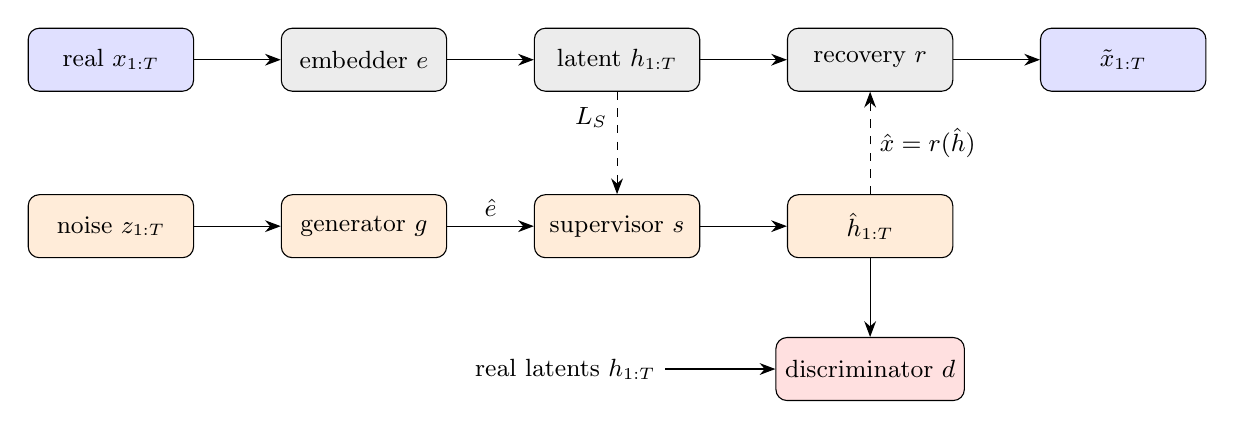
\begin{tikzpicture}[font=\small, node distance=0.6cm and 1.1cm,
    box/.style={draw, rounded corners, minimum width=2.1cm, minimum height=0.8cm, align=center},
    arr/.style={-{Stealth[length=2mm]}}]
    \node[box, fill=blue!12] (x) {real $x_{1:T}$};
    \node[box, fill=gray!15, right=of x] (e) {embedder $e$};
    \node[box, fill=gray!15, right=of e] (h) {latent $h_{1:T}$};
    \node[box, fill=gray!15, right=of h] (r) {recovery $r$};
    \node[box, fill=blue!12, right=of r] (xt) {$\tilde{x}_{1:T}$};
    \node[box, fill=orange!15, below=1.3cm of x] (z) {noise $z_{1:T}$};
    \node[box, fill=orange!15, right=of z] (g) {generator $g$};
    \node[box, fill=orange!15, right=of g] (s) {supervisor $s$};
    \node[box, fill=orange!15, right=of s] (hh) {$\hat{h}_{1:T}$};
    \node[box, fill=red!12, below=1.0cm of hh] (d) {discriminator $d$};
    \draw[arr] (x) -- (e); \draw[arr] (e) -- (h); \draw[arr] (h) -- (r); \draw[arr] (r) -- (xt);
    \draw[arr] (z) -- (g); \draw[arr] (g) -- node[above]{$\hat{e}$} (s); \draw[arr] (s) -- (hh);
    \draw[arr] (hh) -- (d);
    \node[left=1.4cm of d] (hreal) {real latents $h_{1:T}$};
    \draw[arr] (hreal) -- (d);
    \draw[arr, dashed] (hh.north) -- node[right]{$\hat{x} = r(\hat{h})$} (r.south);
    \draw[arr, dashed] (h.south) -- node[left, near start]{$L_S$} (s.north);
\end{tikzpicture}
\caption{The five networks of TimeGAN. The supervisor learns the dynamics on real latents ($L_S$) and applies them to the generator output; the discriminator compares real latents $h$ with synthetic latents $\hat{h}$ (and $\hat{e}$).}
\label{fig:w5_timegan}
\end{figure}

\paragraph{Losses.} TimeGAN combines three losses:
\begin{itemize}
    \item \textbf{Reconstruction loss} $L_R = \E\big[\sum_t \|x_t - \tilde{x}_t\|_2\big]$: the recovery network must rebuild the real sequence from its embedding, so the latent space keeps the information of the 14 channels.
    \item \textbf{Unsupervised (adversarial) loss} $L_U = \E\big[\sum_t \log d(h_t)\big] + \E\big[\sum_t \log\big(1 - d(\hat{h}_t)\big)\big]$: the GAN loss in the latent space. The discriminator maximises it; the generator tries to make $d$ classify $\hat{h}$ as real.
    \item \textbf{Supervised loss} $L_S = \E\big[\sum_t \|h_t - s(h_{t-1})\|_2\big]$: the supervisor must predict the next real latent vector. This is the term that teaches the step-to-step dynamics, which the adversarial loss alone does not capture.
\end{itemize}

\paragraph{Training objective.} The autoencoder is trained so that the latent space is both reconstructible and predictable:
\begin{equation}
\min_{e,\,r} \; \lambda L_S + L_R ,
\end{equation}
and the generator and discriminator play the adversarial game with the supervised loss as a regulariser:
\begin{equation}
\min_{g,\,s} \Big( \eta L_S + \max_{d} L_U \Big),
\end{equation}
where $\lambda$ and $\eta$ are hyperparameters \cite{yoon2019}. Training has three phases: (1) the autoencoder alone on $L_R$, (2) the supervisor alone on $L_S$ with real latents, and (3) the joint phase with all networks.

\paragraph{Implementation.} We ported the official TensorFlow code to PyTorch (\path{models/TimeGAN.py}) and kept its details. All networks are GRUs with 3 layers and hidden size 56 ($4 \times 14$ channels); like the official code, the discriminator is unidirectional. The official loss of the joint phase has the weights $\lambda = 0.1$ and $\eta = 100$ (written as $10\sqrt{L_R} + 0.1 L_S$ for the autoencoder and $L_U + \gamma L_U^{e} + 100\sqrt{L_S} + 100 L_V$ for the generator, where $L_U^{e}$ is the adversarial loss on $\hat{e}$ and $L_V$ matches the batch mean and standard deviation of each channel and day). In every joint iteration the generator is updated twice and the discriminator once, and the discriminator is updated only while its loss is above 0.15.

\subsection{Wasserstein TimeGAN}
\label{sec:w5_wgan}

The Wasserstein GAN replaces the discriminator with a \textbf{critic} $c$ that outputs a real-valued score instead of a probability \cite{arjovsky2017}. The difference between the mean score of real and synthetic samples estimates the Wasserstein-1 distance (earth mover's distance) between the two distributions: the cost of moving the mass of one distribution onto the other. This distance keeps giving the generator a useful gradient when the two distributions do not overlap, which is where the cross-entropy saturates, and it grows when a region of the real data has no synthetic counterpart, so leaving out a type of customer has a cost. The critic must be 1-Lipschitz. WGAN-GP enforces it with a penalty on the gradient norm at random mixtures of real and synthetic samples \cite{gulrajani2017}:
\begin{equation}
L_c = \E\big[c(\hat{h})\big] - \E\big[c(h)\big] + \lambda_{gp}\, \E_{\bar{h}}\Big[\big(\|\nabla_{\bar{h}}\, c(\bar{h})\|_2 - 1\big)^2\Big], \qquad \bar{h} = \epsilon h + (1-\epsilon)\hat{h}, \; \epsilon \sim U(0,1).
\end{equation}
The generator minimises $-\E[c(\hat{h})]$.

In TimeGAN we change only the adversarial part of the joint phase (\path{models/WTimeGAN.py}). The embedder, recovery, generator, supervisor, the first two phases, $L_S$ and $L_V$ stay the same. The critic has no sigmoid and scores a customer with the mean of its per-day outputs. The critic loss uses $\hat{h}$ and $\hat{e}$, each with its own penalty, and the generator loss replaces the two cross-entropy terms with $-c(\hat{h}) - c(\hat{e})$. Following WGAN-GP, the critic takes $n_{\text{critic}} = 5$ steps per generator step, $\lambda_{gp} = 10$, and the rule that pauses the discriminator below a loss of 0.15 is removed.

\paragraph{First approach: recurrent critic (v1).} The direct translation keeps the discriminator network of TimeGAN, a GRU, as the critic. The gradient penalty differentiates the critic twice (the gradient of the gradient norm), and cuDNN, the GPU library that runs recurrent networks efficiently in PyTorch, has no double backward for them. The penalty therefore runs the GRU with cuDNN disabled, one day at a time. On our GPU (RTX 3050) one critic step with the penalty takes 273\,ms, and about 83\,\% of the training time goes to the critic. To keep the run near one hour per class, v1 was trained with 2{,}000 joint iterations, which gives the critic as many updates as the TimeGAN discriminator, and with the WGAN-GP learning rate of $10^{-4}$. The generator then receives about 1\,\% of the TimeGAN update budget (Table~\ref{tab:w5_hparams}), and v1 was very inefficient: giving it a TimeGAN-sized budget with that critic would take about 9 hours per class.

\paragraph{Second approach: convolutional critic (v2).} We replaced the recurrent critic with a temporal convolutional network (TCN): six one-dimensional convolutions over the 90 days, with kernel size 3, dilations $1, 2, 4, 8, 16, 32$, 64 channels and LeakyReLU activations. The receptive field is $1 + 2 \cdot 63 = 127$ days, so every output sees the whole sequence; the convolutions are not causal, so every day is judged with its past and its future, as in the bidirectional discriminator of the paper. There is no batch normalisation, because it mixes customers of the batch and breaks the per-sample penalty. Convolutions support the double backward with cuDNN enabled, and one critic step takes 24\,ms, 11 times faster than the GRU critic.

The change is supported by the literature. TimeGAN places no restriction on the discriminator architecture and mentions temporal convolutions as an alternative for its networks \cite{yoon2019}. The WGAN-GP paper itself uses a one-dimensional CNN critic for sequences in its character-level language model \cite{gulrajani2017}, and WaveGAN trains a one-dimensional convolutional discriminator with WGAN-GP on raw audio \cite{donahue2019}. A recurrent generator with a convolutional discriminator has been used for ECG generation \cite{zhu2019}, Quant GANs use TCNs as discriminator for financial time series \cite{wiese2020}, and TCNs match or outperform LSTMs and GRUs on a wide range of sequence tasks \cite{bai2018}. The critic only interacts with the rest of TimeGAN through the score it gives to a latent sequence, so the generator does not depend on how that score is computed.

With the cheaper critic we gave the generator a full budget: 10{,}000 joint iterations, as TimeGAN, and the Adam learning rate that TimeGAN uses for its generator ($10^{-3}$). The critic keeps the WGAN-GP settings.

% ─────────────────────────────────────────────
\section{Training}
\label{sec:w5_training}
% ─────────────────────────────────────────────

\subsection{Hyperparameters}

Table~\ref{tab:w5_hparams} lists the configuration of the three models. It was set by hand, without a search, and it is the configuration used in the rest of the report; Section~\ref{sec:w5_robustness} repeats the comparison of TimeGAN and v2 with a small search and five seeds. TimeGAN uses the defaults of its paper and WGAN-GP the defaults of its paper. For v2 the generator learning rate and the length of the joint phase were set from the analysis of v1 and a short pilot run on churners (1{,}000 iterations in each of the first two phases and 600 joint iterations): with the TCN critic and a generator learning rate of $10^{-4}$, the norm of the generator weights went from 17.9 to 18.3 and the synthetic customers barely differed from each other, while with $10^{-3}$ the norm reached 21.5 and the moment loss $L_V$ fell from 0.31 to 0.07. All runs use the seed 110.

\begin{table}[H]
\centering
\renewcommand{\arraystretch}{1.3}
\begin{tabularx}{\textwidth}{|P{3.3cm}|Y|Y|Y|}
\hline
 & \textbf{TimeGAN} & \textbf{Wasserstein TimeGAN v1} & \textbf{Wasserstein TimeGAN v2} \\ \hline
Embedder, recovery, generator, supervisor & \multicolumn{3}{c|}{GRU, 3 layers (supervisor: 2), hidden size 56, sigmoid output} \\ \hline
Discriminator / critic & GRU, 3 layers, sigmoid cross-entropy & GRU, 3 layers, raw score (cuDNN off in the penalty) & TCN, 6 dilated Conv1D layers, 64 channels, raw score \\ \hline
Adversarial loss & Binary cross-entropy & WGAN-GP, $\lambda_{gp} = 10$ & WGAN-GP, $\lambda_{gp} = 10$ \\ \hline
Batch size & \multicolumn{3}{c|}{128} \\ \hline
Embedding and supervised phases & \multicolumn{3}{c|}{10{,}000 iterations each, Adam (lr $10^{-3}$)} \\ \hline
Joint iterations & 10{,}000 & 2{,}000 & 10{,}000 \\ \hline
Updates per joint iteration & 2 generator, 1 discriminator (if its loss $> 0.15$) & 1 generator, 5 critic & 1 generator, 5 critic \\ \hline
Generator optimiser & Adam, lr $10^{-3}$ & Adam, lr $10^{-4}$, $\beta = (0.5, 0.9)$ & Adam, lr $10^{-3}$, $\beta = (0.5, 0.9)$ \\ \hline
Critic optimiser & Adam, lr $10^{-3}$ & Adam, lr $10^{-4}$, $\beta = (0.5, 0.9)$ & Adam, lr $10^{-4}$, $\beta = (0.5, 0.9)$ \\ \hline
Generator updates $\times$ lr (relative to TimeGAN) & 1 & 0.01 & 0.5 \\ \hline
Critic step with penalty & -- & 273\,ms & 24\,ms \\ \hline
Training time per class & 27.5\,min & 55\,min & 41.5\,min \\ \hline
\end{tabularx}
\caption{Configuration of the three GANs. Times measured on an RTX 3050; each class is a separate model.}
\label{tab:w5_hparams}
\end{table}

v2 trains five times more joint iterations than v1, each with five critic steps, and still takes 14 minutes less per class.

\subsection{Convergence}

Figures~\ref{fig:w5_hist_timegan} to~\ref{fig:w5_hist_v2} show the losses of the three models for the churners (the non-churner curves are in \path{docs/w5/figures/}). The first two phases behave the same in every model, because they are identical: the reconstruction loss falls from 0.42 to about 0.03 and the supervised loss settles around 0.12.

\begin{figure}[H]
\centering
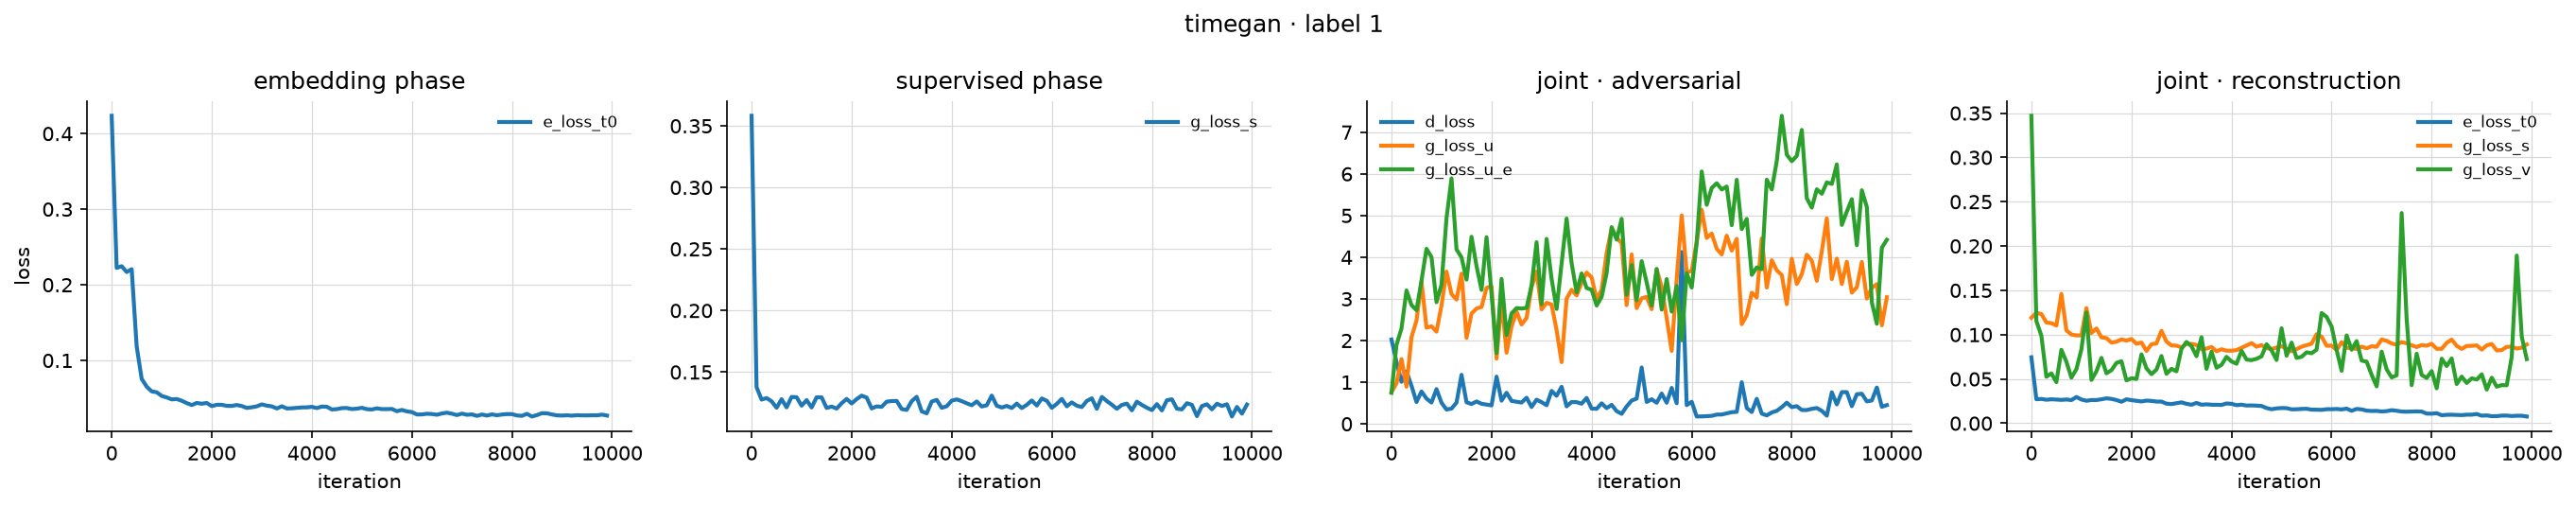
\includegraphics[width=\textwidth]{figures/gan_models/history/timegan_history_label1.png}
\caption{TimeGAN, churners. In the joint phase the discriminator loss stays mostly below 1 while the generator adversarial losses $L_U$ and $L_U^{e}$ rise from 0.8 to between 3 and 7.}
\label{fig:w5_hist_timegan}
\end{figure}

\begin{figure}[H]
\centering
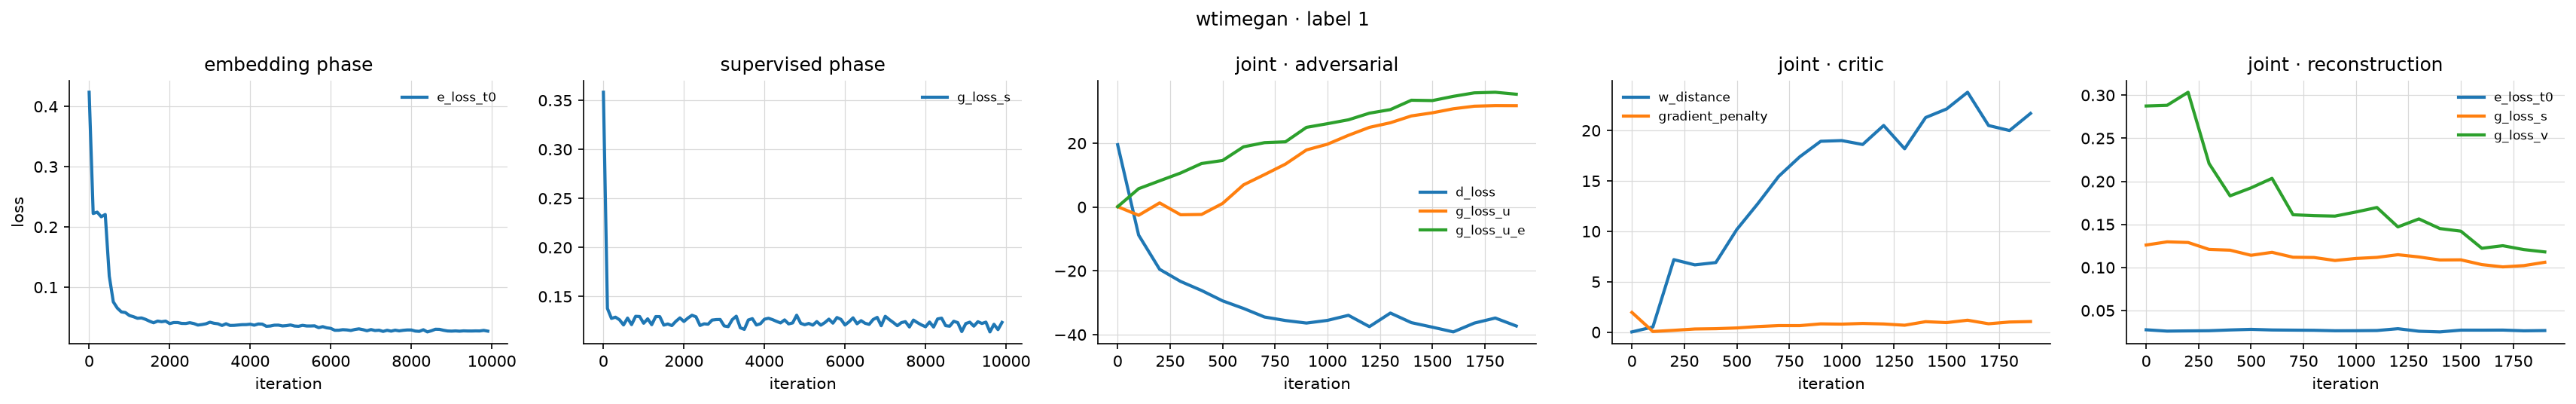
\includegraphics[width=\textwidth]{figures/gan_models/history/wtimegan_history_label1.png}
\caption{Wasserstein TimeGAN v1, churners (2{,}000 joint iterations). The estimated Wasserstein distance rises from 0 to about 22 and is still rising at the end of the run.}
\label{fig:w5_hist_v1}
\end{figure}

\begin{figure}[H]
\centering
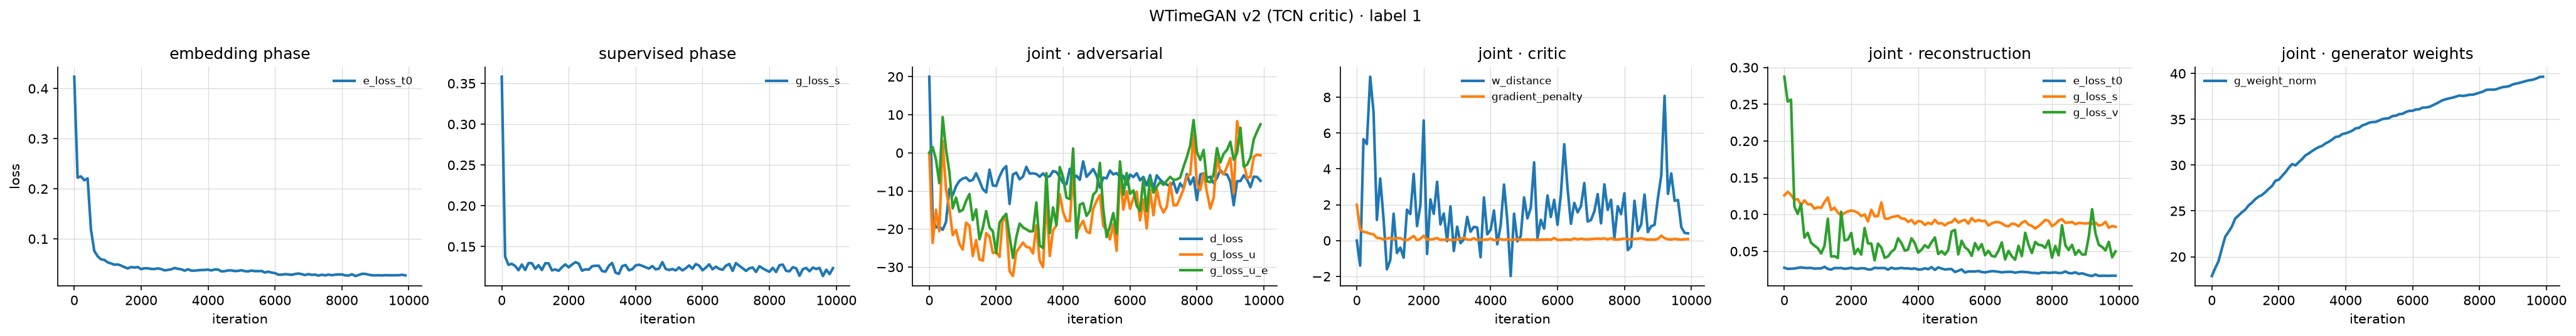
\includegraphics[width=\textwidth]{figures/wgan_tcn/history/history_label1.png}
\caption{Wasserstein TimeGAN v2, churners. The estimated Wasserstein distance peaks early and then stays between about 0 and 2 with occasional spikes; the gradient penalty stays near 0; the norm of the generator weights grows steadily from 17.9 to about 40.}
\label{fig:w5_hist_v2}
\end{figure}

\paragraph{TimeGAN.} The discriminator wins the game. Its loss drops from 2.0 to values between 0.2 and 0.8 while the generator adversarial loss climbs (Table~\ref{tab:w5_timegan_dyn}). With a cross-entropy discriminator that is confident, the generator gradient becomes small, which is the vanishing-gradient situation that motivated the Wasserstein loss. The discriminator was updated in every logged step, so the 0.15 rule never paused it.

\begin{table}[H]
\centering
\renewcommand{\arraystretch}{1.3}
\begin{adjustbox}{max width=\textwidth}
\begin{tabular}{|r|r|r|r|r|}
\hline
 & \multicolumn{2}{c|}{\textbf{Churners}} & \multicolumn{2}{c|}{\textbf{Non-churners}} \\ \hline
\textbf{Joint iteration} & \textbf{$d$ loss} & \textbf{$g$ loss $L_U$} & \textbf{$d$ loss} & \textbf{$g$ loss $L_U$} \\ \hline
0     & 2.02 & 0.76 & 2.02 & 0.75 \\ \hline
2{,}500 & 0.53 & 2.70 & 0.31 & 3.81 \\ \hline
5{,}000 & 1.35 & 3.01 & 0.36 & 5.32 \\ \hline
7{,}500 & 0.20 & 3.27 & 0.23 & 5.98 \\ \hline
9{,}900 & 0.45 & 3.04 & 0.60 & 2.80 \\ \hline
\end{tabular}
\end{adjustbox}
\caption{Adversarial losses of TimeGAN in the joint phase.}
\label{tab:w5_timegan_dyn}
\end{table}

\paragraph{Wasserstein TimeGAN.} In a healthy WGAN-GP run the estimated distance rises while the critic learns and then comes down as the generator catches up. In v1 it only rises (Table~\ref{tab:w5_wdist}): within its 2{,}000 generator updates at $10^{-4}$ the generator does not catch up with the critic. In v2 the distance stays low for the whole run. The generator weights show the difference in progress: their norm moves from 17.9 to 18.5 in v1, and to about 40 (churners) and 36 (non-churners) in v2, comparable to the 48 to 50 of TimeGAN. The moment loss $L_V$ is also lower in v2 (about 0.05 against 0.12 to 0.14 at the end of v1).

\begin{table}[H]
\centering
\renewcommand{\arraystretch}{1.3}
\begin{adjustbox}{max width=\textwidth}
\begin{tabular}{|l|r|r|r|r|r|}
\hline
\textbf{Model} & \multicolumn{5}{c|}{\textbf{Mean estimated Wasserstein distance per block of the joint phase}} \\ \hline
\multirow{2}{*}{v1 (churners)} & it. 0--499 & 500--999 & 1{,}000--1{,}499 & 1{,}500--1{,}999 & \\ \cline{2-6}
 & 4.3 & 14.9 & 19.5 & 21.6 & \\ \hline
\multirow{2}{*}{v2 (churners)} & it. 0--1{,}999 & 2{,}000--3{,}999 & 4{,}000--5{,}999 & 6{,}000--7{,}999 & 8{,}000--9{,}999 \\ \cline{2-6}
 & 1.9 & 1.1 & 1.2 & 2.0 & 1.8 \\ \hline
\multirow{2}{*}{v2 (non-churners)} & it. 0--1{,}999 & 2{,}000--3{,}999 & 4{,}000--5{,}999 & 6{,}000--7{,}999 & 8{,}000--9{,}999 \\ \cline{2-6}
 & 2.5 & 1.0 & 0.9 & 1.7 & 1.6 \\ \hline
\end{tabular}
\end{adjustbox}
\caption{Estimated Wasserstein distance between real and synthetic latents (one batch per logged step). v1 for non-churners behaves like v1 for churners, peaking at 16.}
\label{tab:w5_wdist}
\end{table}

A small Wasserstein estimate alone could also mean a weak critic, so the convergence curves have to be read together with the quality metrics of the next section.

\subsection{Hyperparameter Search and Seed Variability}
\label{sec:w5_robustness}

The results of Section~\ref{sec:w5_quality} come from one run per model with the seed 110 and a hand-set configuration. To check that the advantage of v2 over TimeGAN does not depend on that run, we repeated the training of both models in two steps (\path{workshops/w5/run_experiments.py}).

\paragraph{Search.} For each GAN and each class we ran 15 Optuna trials (TPE sampler) with a reduced budget: 1{,}000 iterations per phase, and 600 joint iterations for v2. The search space covers the hidden size (28, 56 or 84), the number of layers (2 to 4) and the learning rates (TimeGAN: $3\cdot10^{-4}$ to $3\cdot10^{-3}$; v2: generator $3\cdot10^{-4}$ to $3\cdot10^{-3}$, critic $3\cdot10^{-5}$ to $3\cdot10^{-4}$, and 3 or 5 critic steps). The objective is the Fréchet distance of Section~\ref{sec:w5_quality}, and the hand-set configuration is the first trial, so the search can only match or improve it. Table~\ref{tab:w5_optuna} lists the best configurations. Both TimeGAN searches used the same sampler seed, so they proposed the same candidates, and the same one won in both classes.

\begin{table}[H]
\centering
\renewcommand{\arraystretch}{1.3}
\begin{adjustbox}{max width=\textwidth}
\begin{tabular}{|l|c|r|r|r|r|r|}
\hline
\textbf{GAN} & \textbf{Class} & \textbf{Hidden} & \textbf{Layers} & \textbf{Generator lr} & \textbf{Critic lr} & \textbf{Critic steps} \\ \hline
TimeGAN & both & 28 & 2 & $7.8\cdot10^{-4}$ & -- & -- \\ \hline
v2 & churners & 28 & 4 & $1.6\cdot10^{-3}$ & $6.4\cdot10^{-5}$ & 3 \\ \hline
v2 & non-churners & 84 & 4 & $3.1\cdot10^{-4}$ & $3.1\cdot10^{-5}$ & 3 \\ \hline
\end{tabular}
\end{adjustbox}
\caption{Best configurations found by the search (hand-set configuration: hidden size 56, 3 layers, lr $10^{-3}$; v2 critic lr $10^{-4}$ and 5 critic steps).}
\label{tab:w5_optuna}
\end{table}

\paragraph{Seeds.} Each model was then retrained with its best configuration and the full budget of Table~\ref{tab:w5_hparams} with five seeds (0 to 4), and evaluated exactly as in Section~\ref{sec:w5_quality}. The 20 runs took about 13 hours in total.

\begin{table}[H]
\centering
\renewcommand{\arraystretch}{1.3}
\begin{adjustbox}{max width=\textwidth}
\begin{tabular}{|c|l|r|r|r|r|r|}
\hline
\textbf{Class} & \textbf{GAN} & \textbf{Fréchet} & \textbf{Fréchet, single run} & \textbf{Discrim.} & \textbf{Predictive} & \textbf{Own class} \\ \hline
\multirow{2}{*}{Churners} & TimeGAN & $0.454 \pm 0.078$ & 0.936 & $0.485 \pm 0.007$ & $0.093 \pm 0.015$ & 82\% \\ \cline{2-7}
 & Wasserstein v2 & $\mathbf{0.224 \pm 0.092}$ & 0.247 & $\mathbf{0.411 \pm 0.054}$ & $0.093 \pm 0.012$ & 87\% \\ \hline
\multirow{2}{*}{Non-churners} & TimeGAN & $0.402 \pm 0.238$ & 0.091 & $0.494 \pm 0.004$ & $0.100 \pm 0.004$ & 30\% \\ \cline{2-7}
 & Wasserstein v2 & $\mathbf{0.194 \pm 0.214}$ & 0.029 & $\mathbf{0.472 \pm 0.014}$ & $0.092 \pm 0.006$ & 45\% \\ \hline
\end{tabular}
\end{adjustbox}
\caption{Mean $\pm$ standard deviation over five seeds with the configurations of Table~\ref{tab:w5_optuna}. Single run: hand-set configuration, seed 110 (Table~\ref{tab:w5_quality}). Metrics as in Table~\ref{tab:w5_quality}.}
\label{tab:w5_seeds}
\end{table}

\begin{figure}[H]
\centering
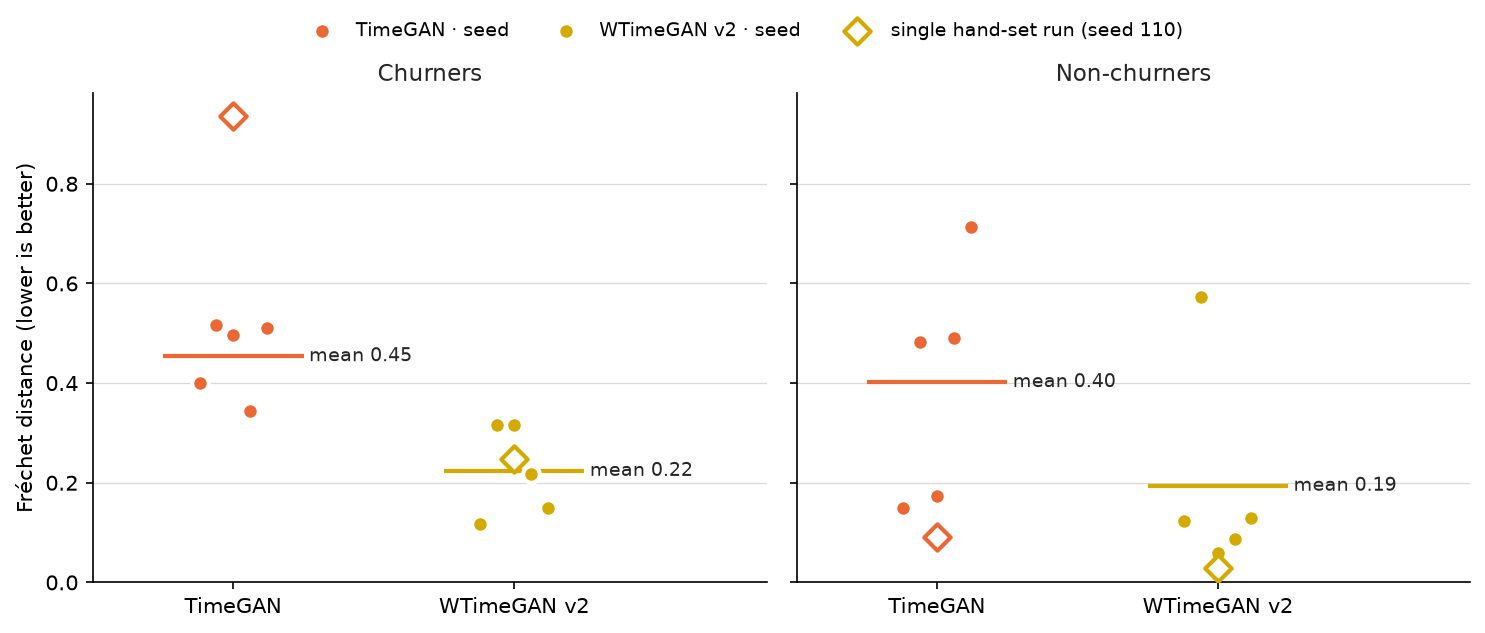
\includegraphics[width=\textwidth]{figures/experiments/frechet_seeds.png}
\caption{Fréchet distance of each of the five seeds (dots) and their mean (line), with the tuned configurations. The diamond is the single hand-set run of Table~\ref{tab:w5_quality}.}
\label{fig:w5_frechet_seeds}
\end{figure}

\paragraph{v2 against TimeGAN.} The advantage of v2 holds across seeds (Table~\ref{tab:w5_seeds}). Its mean Fréchet distance is about half that of TimeGAN in both classes, its discriminative score is lower in both, and in the comparison seed by seed v2 has the lower Fréchet distance in 9 of the 10 pairs (5 of 5 for churners, 4 of 5 for non-churners). The predictive score does not separate the two models. Neither model fools the post-hoc discriminator (scores between 0.41 and 0.49), so the conclusion is about relative quality, not about indistinguishable customers.

\paragraph{Search against the hand-set configuration.} For the churners the search clearly helped TimeGAN: the mean Fréchet distance falls from 0.94 in the single run to 0.45, and all five seeds are below 0.52. For v2 it brought nothing: the mean of 0.22 matches the 0.25 of the single run, which therefore was not a lucky seed. For the non-churners the search did not carry over to the full budget. The tuned configurations give a worse Fréchet distance than the single hand-set run (TimeGAN 0.40 against 0.09; v2 0.19 against 0.03), with a large spread between seeds (TimeGAN from 0.15 to 0.71). The single run lies below all five tuned seeds for both models, which suggests that the hand-set configuration is better for this class. It is still one run against five, so we did not confirm it with several seeds of the hand-set configuration. The likely cause is the reduced budget of the search: a configuration that is best after 1{,}000 iterations need not be best after 10{,}000. The spread between seeds also shows that a single run is not enough to rank configurations, which is why this section reports means and standard deviations.

% ─────────────────────────────────────────────
\section{Generation Quality}
\label{sec:w5_quality}
% ─────────────────────────────────────────────

\subsection{Metrics}

Every metric compares the synthetic customers of one class with the real \texttt{fit} customers of that class and reports the same metric for the real \texttt{tune} customers, which the GAN never saw. A synthetic score close to the \texttt{tune} score means the GAN is as close to the training data as a fresh real sample.

\begin{itemize}
    \item \textbf{Fréchet distance.} The recipe of the Fréchet Inception Distance \cite{heusel2017} with the Inception network replaced by the Workshop~2 churn LSTM: each customer is represented by the last hidden state of the LSTM (64 dimensions), a Gaussian is fitted to each set, and $\text{FD} = \|\mu_r - \mu_s\|^2 + \operatorname{Tr}\big(\Sigma_r + \Sigma_s - 2(\Sigma_r \Sigma_s)^{1/2}\big)$. It measures realism as seen by the churn model. Lower is better.
    \item \textbf{Discriminative score} \cite{yoon2019}. A one-layer GRU is trained to separate real from synthetic customers (balanced, 80/20 split, 2{,}000 steps) and the score is $|\text{accuracy} - 0.5|$ on the held-out part: 0 means indistinguishable, 0.5 means trivially separable.
    \item \textbf{Predictive score} \cite{yoon2019}. A one-layer GRU is trained on the synthetic customers to predict day $t+1$ from days $\le t$ and is tested on real \texttt{tune} customers (mean absolute error on the min-max scale). The reference is the same model trained on real \texttt{fit} customers.
    \item \textbf{Churn view.} The mean churn probability that the Workshop~2 LSTM assigns to the synthetic customers, and the share it classifies into their own class at its threshold.
    \item \textbf{Mode-collapse signals.} The share of customers with 0 or at least 85 active days, the median number of switches between active and inactive days, the share without any payment, and two nearest-neighbour distances on the flattened $90 \times 14$ sequences (2{,}000 customers, min-max scale of \texttt{fit}): the median distance of a synthetic customer to the nearest other synthetic customer (diversity) and the median distance of a real \texttt{tune} customer to the nearest synthetic customer (coverage).
\end{itemize}

\subsection{Quantitative Results}

\begin{table}[H]
\centering
\renewcommand{\arraystretch}{1.3}
\begin{adjustbox}{max width=\textwidth}
\begin{tabular}{|c|l|r|r|r|r|r|}
\hline
\textbf{Class} & \textbf{Source} & \textbf{Fréchet} & \textbf{Discrim.} & \textbf{Predictive} & \textbf{Churn prob.} & \textbf{Own class} \\ \hline
\multirow{4}{*}{Churners} & Real \texttt{tune} (reference) & 0.008 & 0.015 & 0.108 & 0.48 & 72\% \\ \cline{2-7}
 & TimeGAN & 0.936 & 0.457 & 0.093 & 0.75 & 91\% \\ \cline{2-7}
 & Wasserstein v1 & 0.837 & 0.496 & 0.130 & 0.31 & 47\% \\ \cline{2-7}
 & Wasserstein v2 & \textbf{0.247} & \textbf{0.390} & 0.073 & \textbf{0.52} & 80\% \\ \hline
\multirow{4}{*}{Non-churners} & Real \texttt{tune} (reference) & 0.001 & 0.001 & 0.092 & 0.25 & 68\% \\ \cline{2-7}
 & TimeGAN & 0.091 & 0.478 & 0.105 & 0.33 & 60\% \\ \cline{2-7}
 & Wasserstein v1 & 0.066 & 0.423 & 0.121 & 0.27 & 56\% \\ \cline{2-7}
 & Wasserstein v2 & \textbf{0.029} & 0.429 & 0.107 & 0.29 & 57\% \\ \hline
\end{tabular}
\end{adjustbox}
\caption{Quality metrics. Fréchet: distance to real \texttt{fit} in the feature space of the Workshop~2 LSTM. Discrim.: discriminative score. Predictive: next-day MAE on real \texttt{tune} of a model trained on each source. Churn prob.: mean churn probability given by the Workshop~2 LSTM. Own class: share classified into the customer's own class. Bold: best GAN where it is clearly ahead.}
\label{tab:w5_quality}
\end{table}

v2 reduces the Fréchet distance of the churners from 0.94 (TimeGAN) to 0.25 and of the non-churners from 0.091 to 0.029. Its synthetic churners receive a mean churn probability of 0.52, close to the 0.48 of real churners, while TimeGAN churners receive 0.75: TimeGAN generated exaggerated churners, and v1 generated churners that the LSTM mostly reads as non-churners (0.31). The discriminative score improves only partly: a small GRU still separates real from v2 customers with about 89 to 93\,\% accuracy, so the synthetic customers are not indistinguishable. The predictive score of TimeGAN and v2 churners is lower than the real reference; smoother synthetic sequences teach a conservative next-day prediction that the MAE rewards, so we do not read it as better than real data.

\begin{table}[H]
\centering
\renewcommand{\arraystretch}{1.3}
\begin{adjustbox}{max width=\textwidth}
\begin{tabular}{|c|l|r|r|r|r|r|r|}
\hline
\textbf{Class} & \textbf{Source} & \textbf{0 days} & \textbf{$\ge$85 days} & \textbf{Switches} & \textbf{No pay} & \textbf{NN within} & \textbf{NN real$\to$synth.} \\ \hline
\multirow{4}{*}{Churners} & Real \texttt{tune} & 4.5\% & 8.5\% & 14 & 28\% & 5.57 & 5.57 \\ \cline{2-8}
 & TimeGAN & 46.5\% & 26.6\% & 0 & 65\% & 0.16 & 7.13 \\ \cline{2-8}
 & Wasserstein v1 & 0.0\% & 0.0\% & 26 & 85\% & 1.09 & 9.08 \\ \cline{2-8}
 & Wasserstein v2 & 1.7\% & 5.8\% & 9 & 46\% & 5.08 & 5.80 \\ \hline
\multirow{4}{*}{Non-churners} & Real \texttt{tune} & 0.2\% & 14.7\% & 17 & 15\% & 6.09 & 6.17 \\ \cline{2-8}
 & TimeGAN & 5.4\% & 8.5\% & 12 & 28\% & 5.94 & 7.16 \\ \cline{2-8}
 & Wasserstein v1 & 0.0\% & 55.9\% & 1 & 83\% & 0.46 & 7.57 \\ \cline{2-8}
 & Wasserstein v2 & 0.6\% & 46.3\% & 6 & 17\% & 4.63 & 6.93 \\ \hline
\end{tabular}
\end{adjustbox}
\caption{Mode-collapse signals. 0 days / $\ge$85 days: share of customers with no active day or with at least 85 of 90. Switches: median number of changes between active and inactive. No pay: share without any payment day. NN within: median distance to the nearest other customer of the same set. NN real$\to$synth.: median distance from a real \texttt{tune} customer to the nearest customer of the set (for the real row, to the nearest \texttt{fit} customer).}
\label{tab:w5_collapse}
\end{table}

For the churners v2 is close to the real reference on most signals: synthetic churners are about as far from each other as real ones (5.08 against 5.57), and a real churner finds a synthetic one almost as close as another real one (5.80 against 5.57). TimeGAN churners are near copies of each other (0.16) and leave real churners uncovered (7.13). For the non-churners the picture is mixed: v2 has the best Fréchet distance, but 46\,\% of its non-churners are active on at least 85 days against 15\,\% of real ones, and they switch between active and inactive 6 times instead of 17.

\subsection{Qualitative Assessment}

\paragraph{Latent projections.} Figures~\ref{fig:w5_emb_1} and~\ref{fig:w5_emb_0} project the LSTM features of real and synthetic customers with PCA and t-SNE, one model at a time. Synthetic points should cover the real cloud, without concentrating in one region and without forming separate islands.

\begin{figure}[H]
\centering
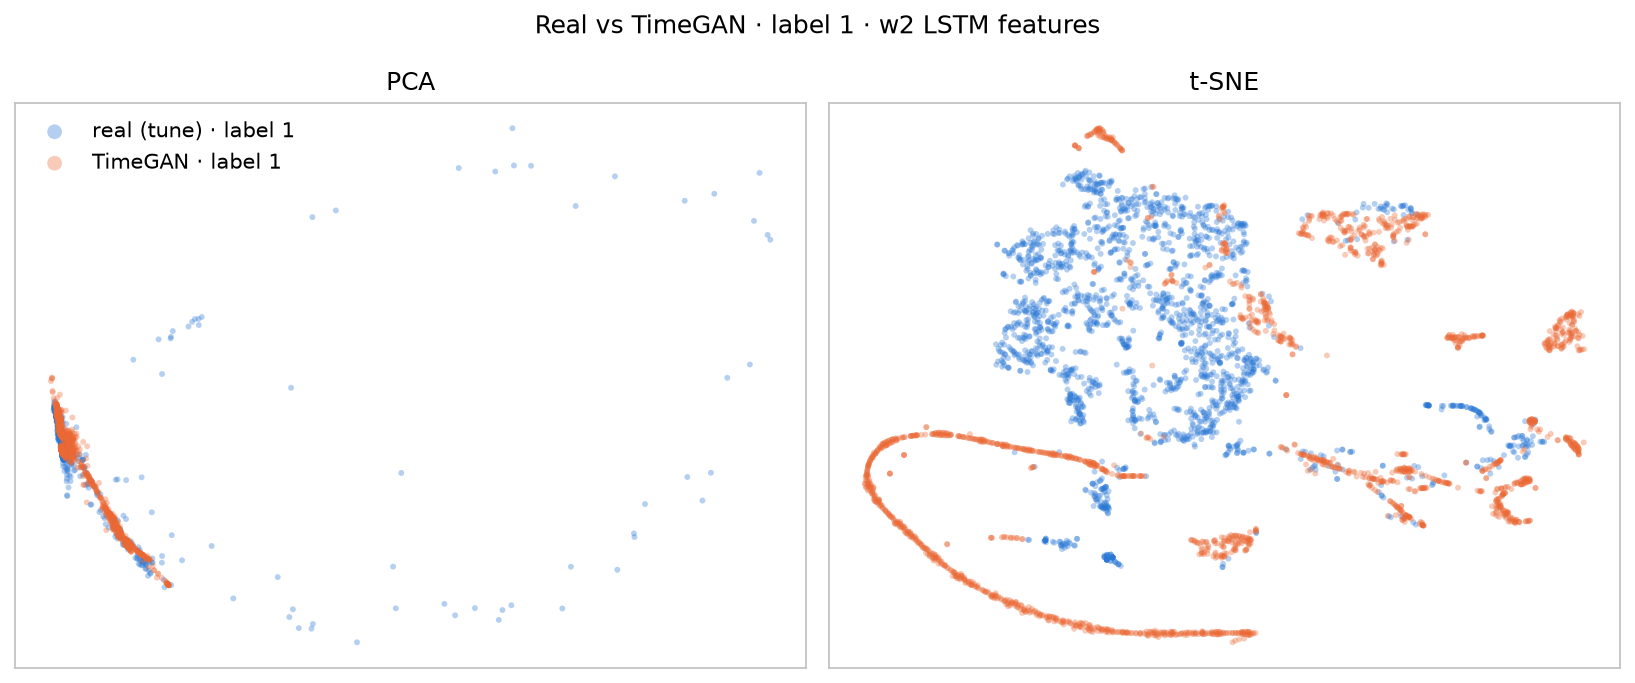
\includegraphics[width=0.92\textwidth]{figures/wgan_tcn/embedding_label1_timegan.png}\\[0.3em]
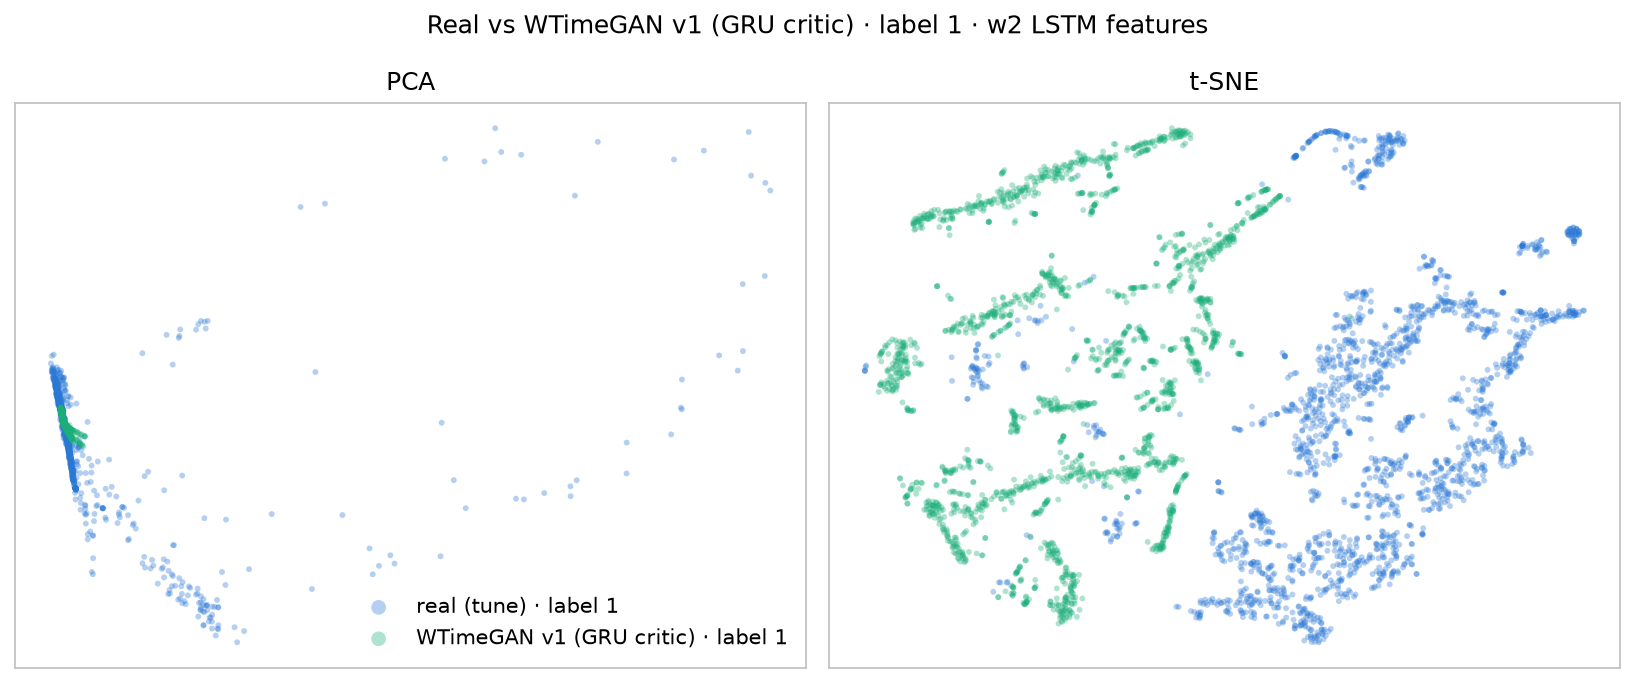
\includegraphics[width=0.92\textwidth]{figures/wgan_tcn/embedding_label1_wtimegan.png}\\[0.3em]
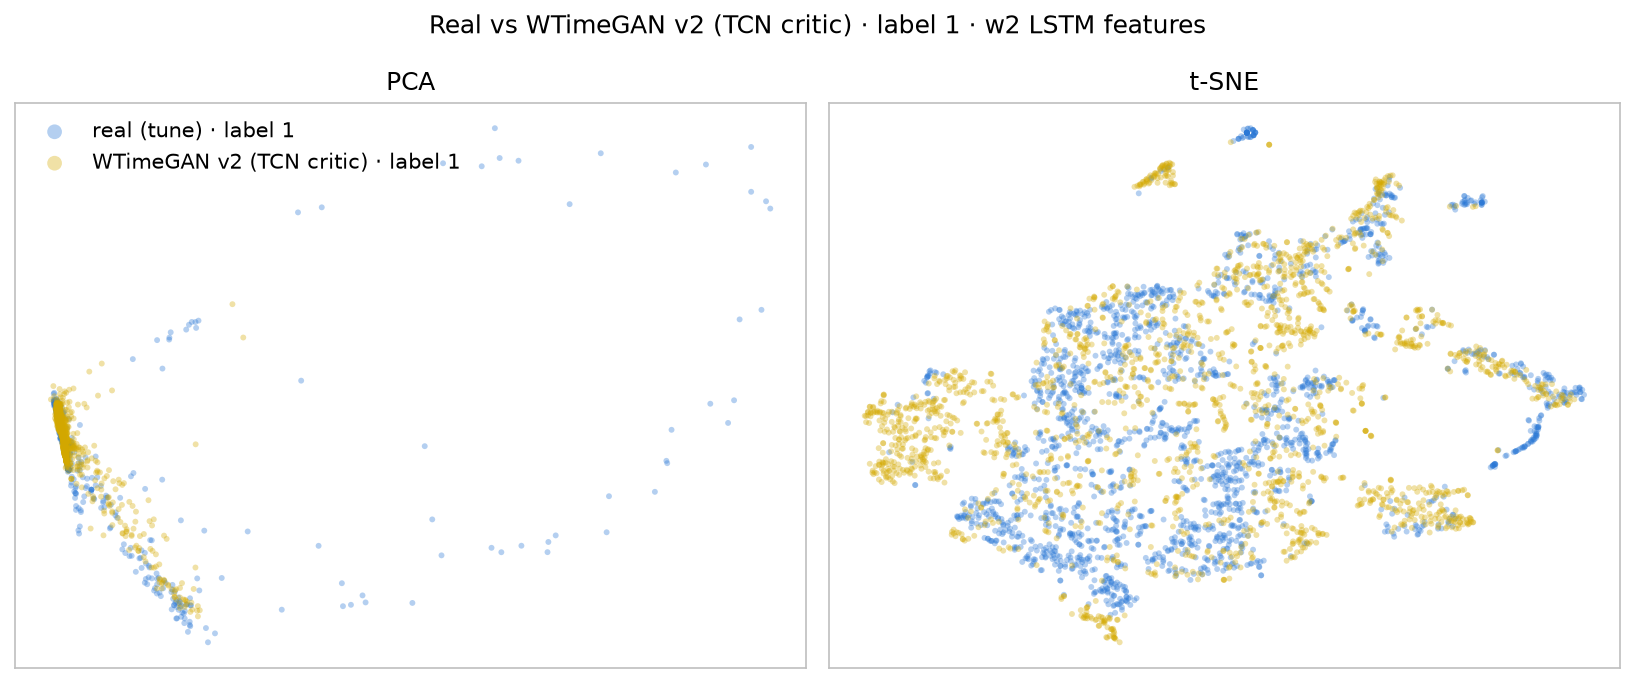
\includegraphics[width=0.92\textwidth]{figures/wgan_tcn/embedding_label1_wtimegan_tcn.png}
\caption{Churners: real (blue) against TimeGAN (top), Wasserstein v1 (middle) and Wasserstein v2 (bottom). TimeGAN forms a long thin curve and separate filaments; v1 forms filaments in a region with no real customers; v2 mixes with the real cloud and covers most of it, with a few synthetic-only islands.}
\label{fig:w5_emb_1}
\end{figure}

\begin{figure}[H]
\centering
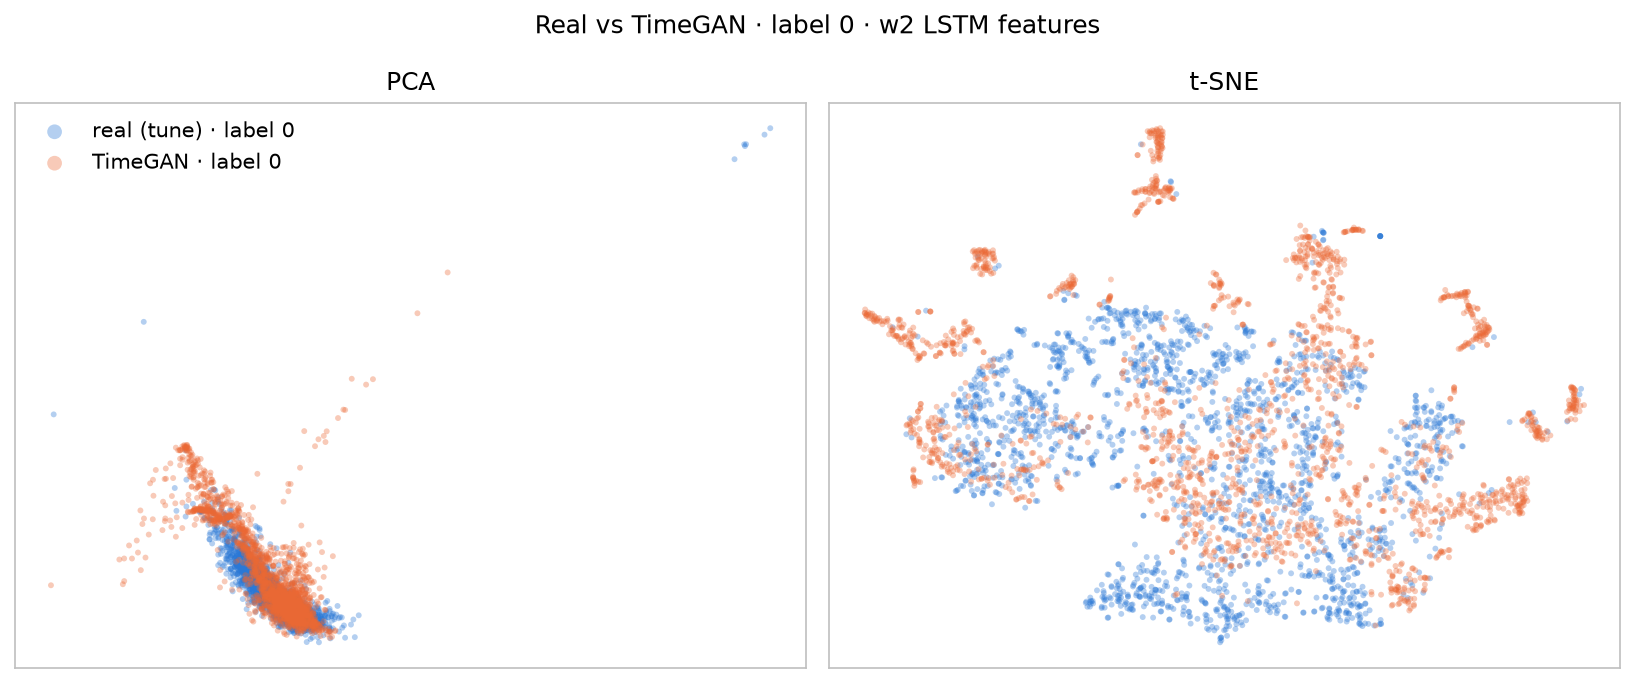
\includegraphics[width=0.92\textwidth]{figures/wgan_tcn/embedding_label0_timegan.png}\\[0.3em]
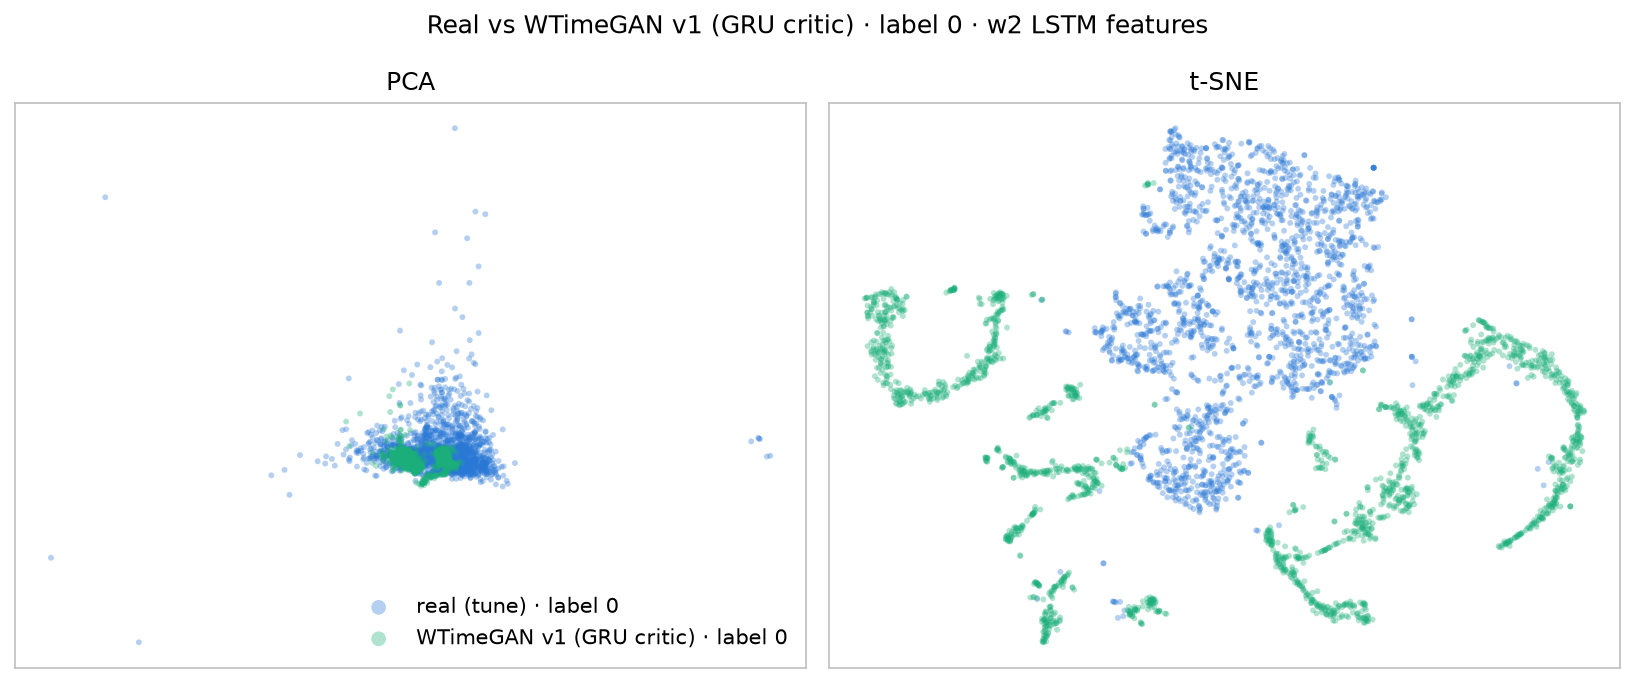
\includegraphics[width=0.92\textwidth]{figures/wgan_tcn/embedding_label0_wtimegan.png}\\[0.3em]
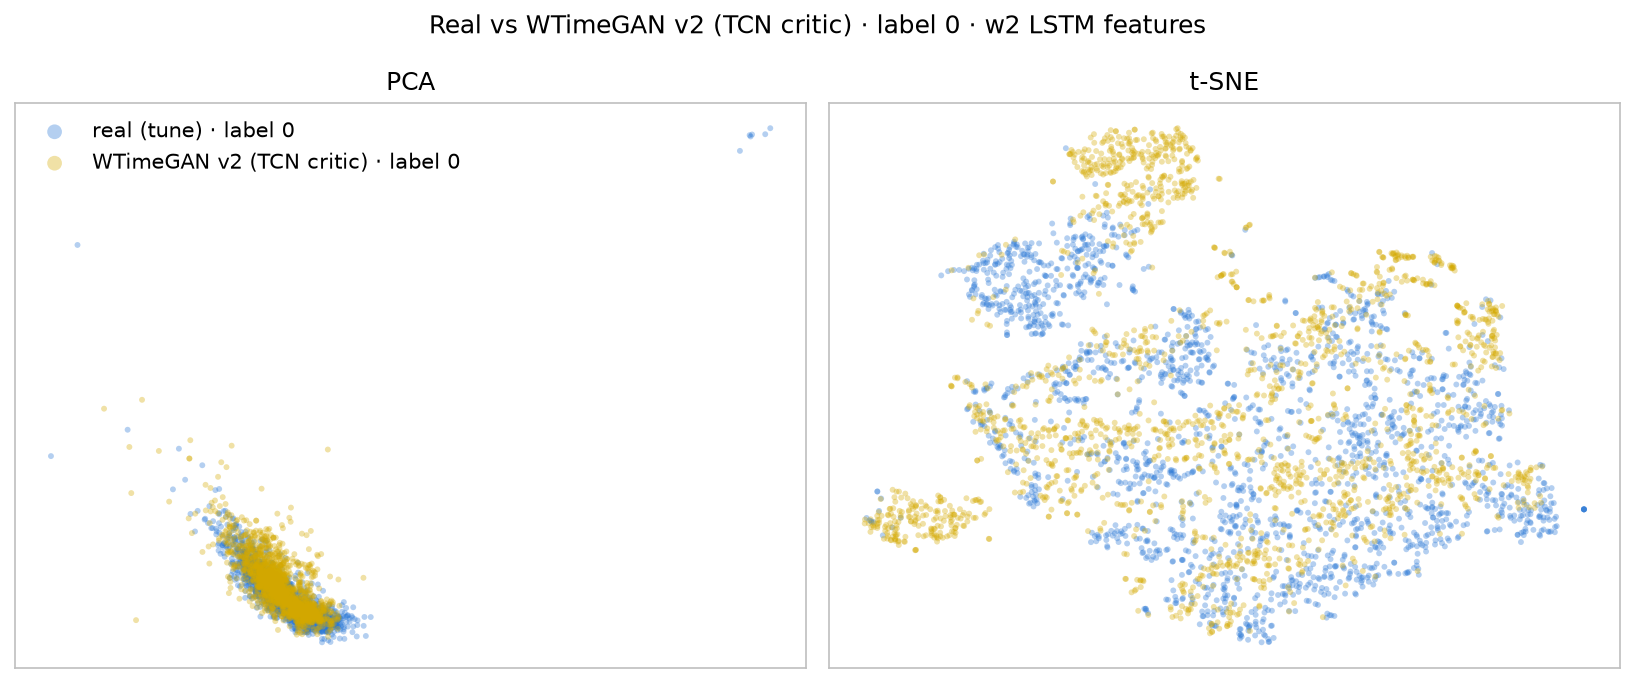
\includegraphics[width=0.92\textwidth]{figures/wgan_tcn/embedding_label0_wtimegan_tcn.png}
\caption{Non-churners: real (blue) against TimeGAN (top), Wasserstein v1 (middle) and Wasserstein v2 (bottom).}
\label{fig:w5_emb_0}
\end{figure}

\paragraph{Daily profiles and aggregates.} Figure~\ref{fig:w5_profiles} shows the mean of each channel per day. v2 follows the real listening curves and the growth of \texttt{tx\_state\_known} over the window, which TimeGAN and v1 fix at 1 from the first days; TimeGAN churners pay on about four times as many days as real churners. Figure~\ref{fig:w5_aggregates} compares per-customer aggregates. For churners the distribution of active days of v2 is almost identical to the real one (Kolmogorov--Smirnov statistic 0.056 against 0.42 for TimeGAN); for non-churners v2 piles customers at 89 to 90 active days.

\begin{figure}[H]
\centering
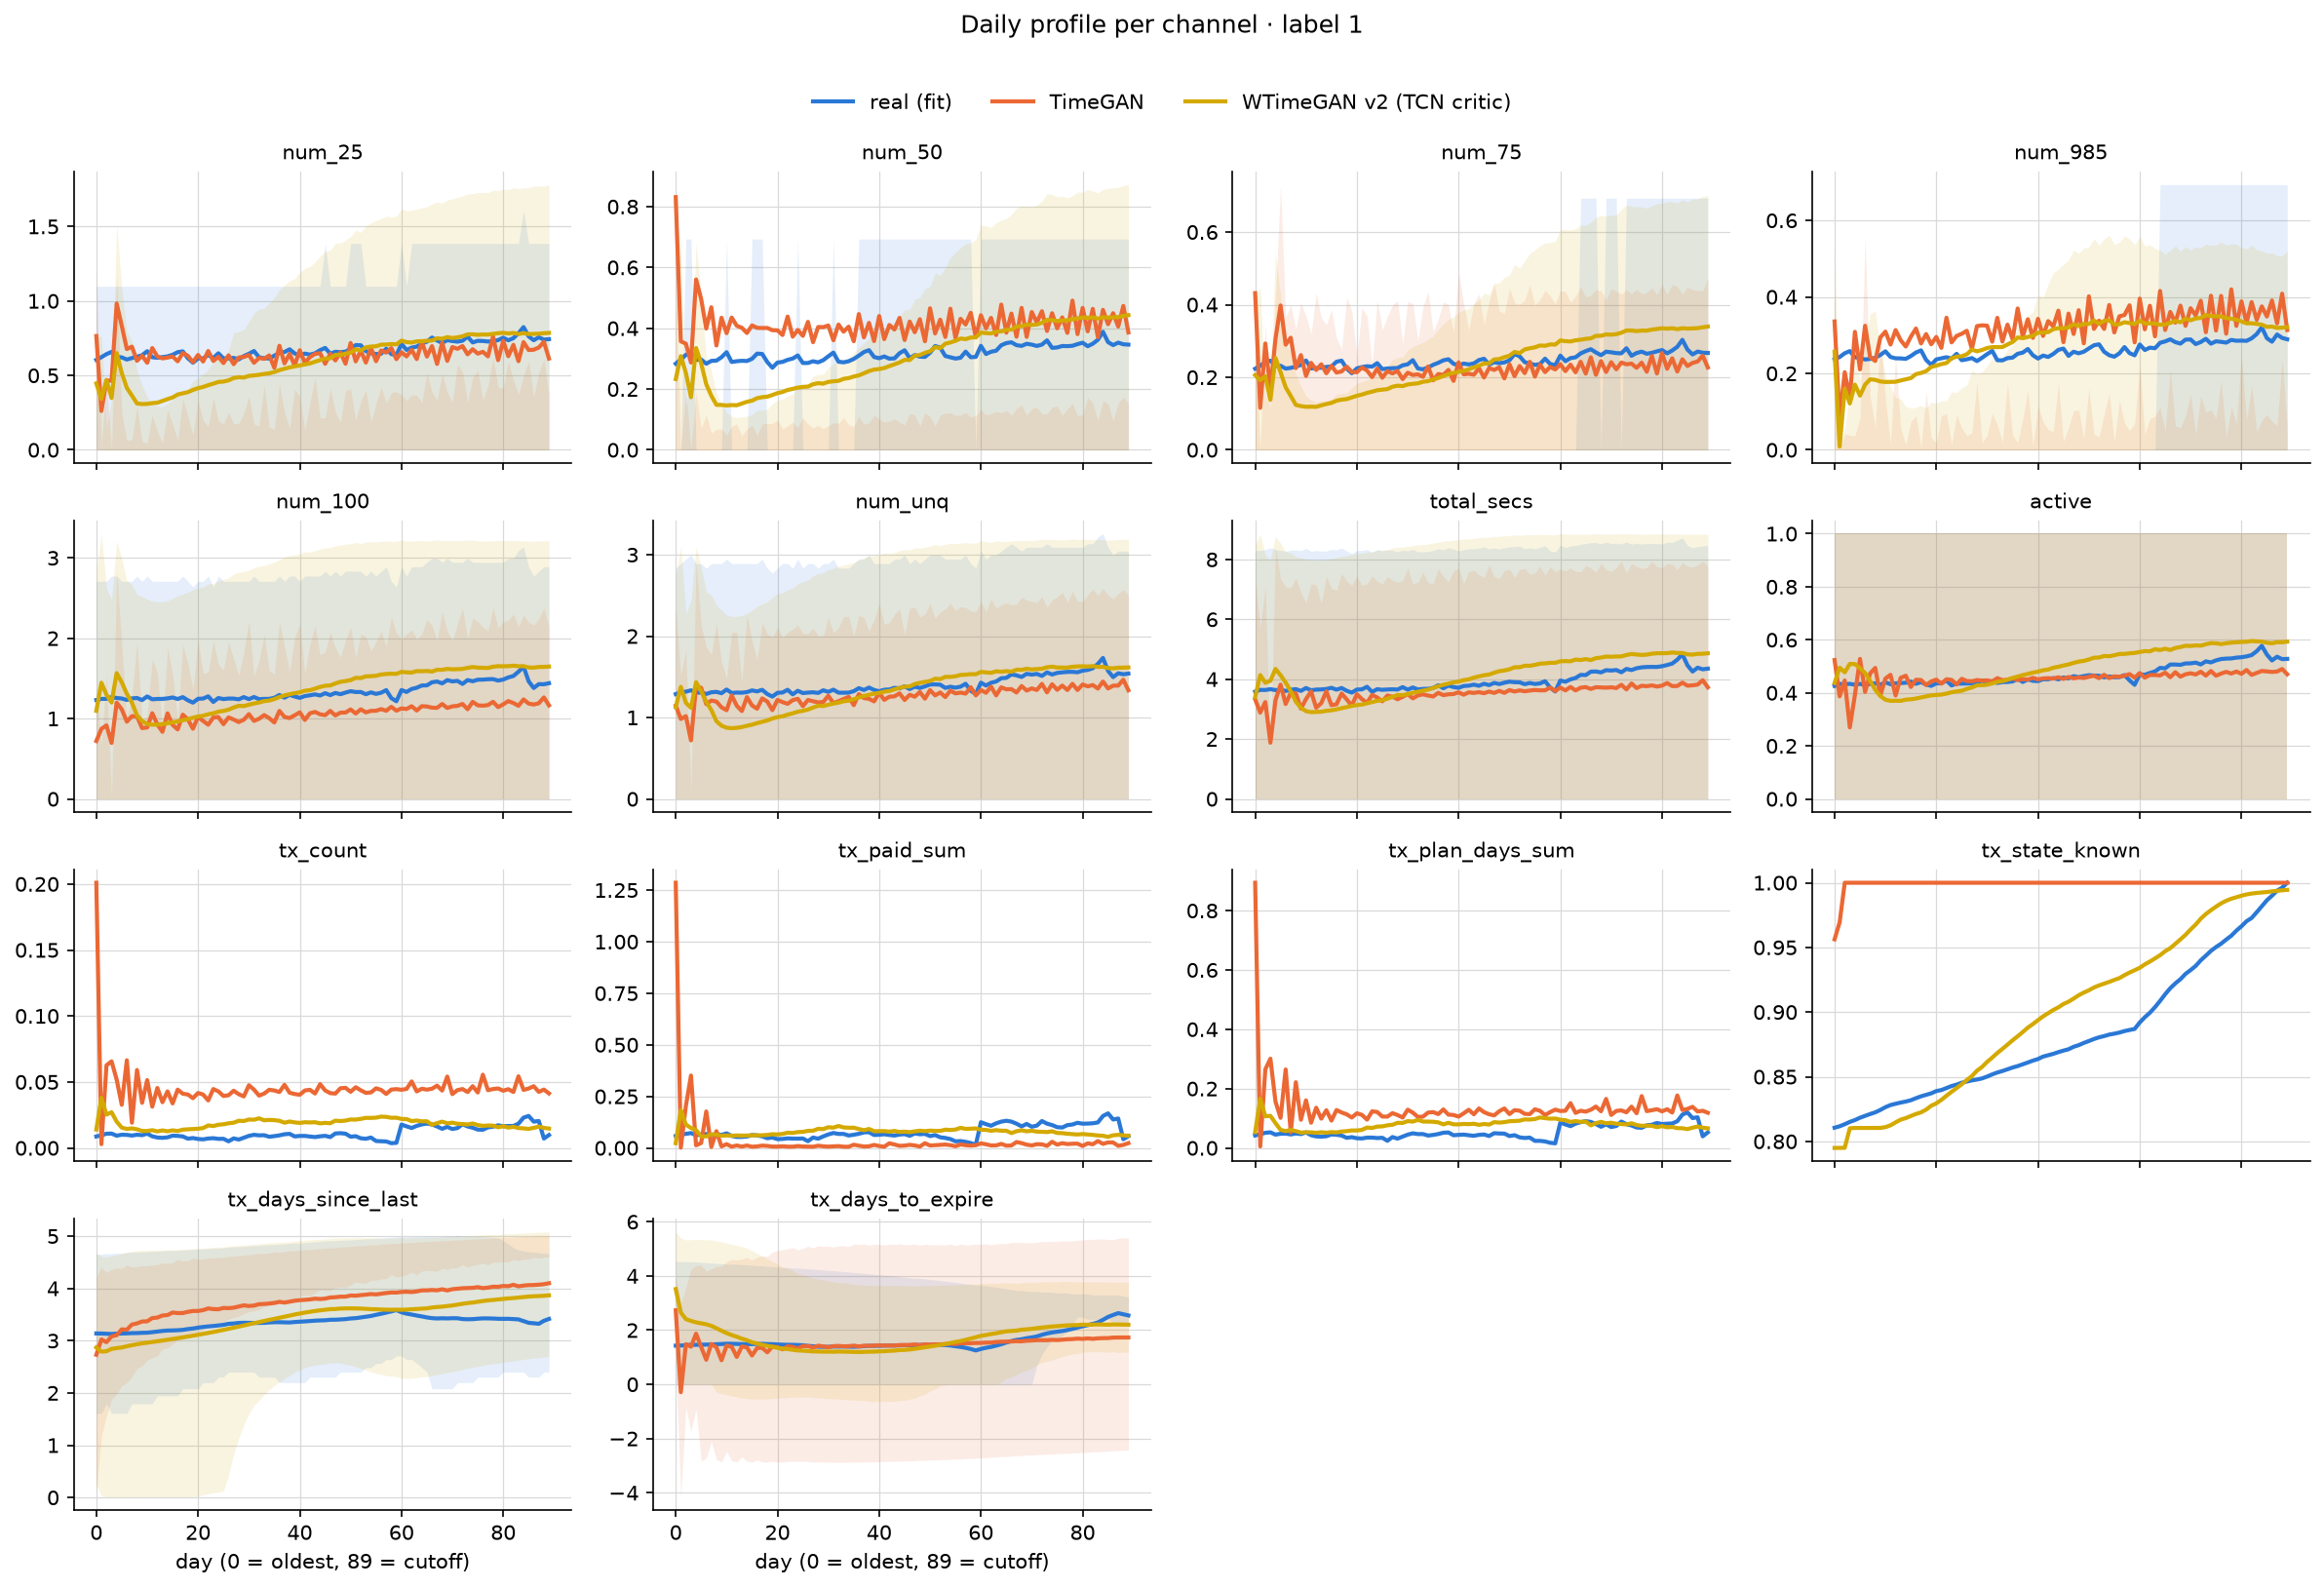
\includegraphics[width=\textwidth]{figures/wgan_tcn/daily_profiles_label1.png}
\caption{Mean and 25 to 75\% band of every channel per day, churners. Real \texttt{fit} in blue, TimeGAN in orange, v1 in green, v2 in gold.}
\label{fig:w5_profiles}
\end{figure}

\begin{figure}[H]
\centering
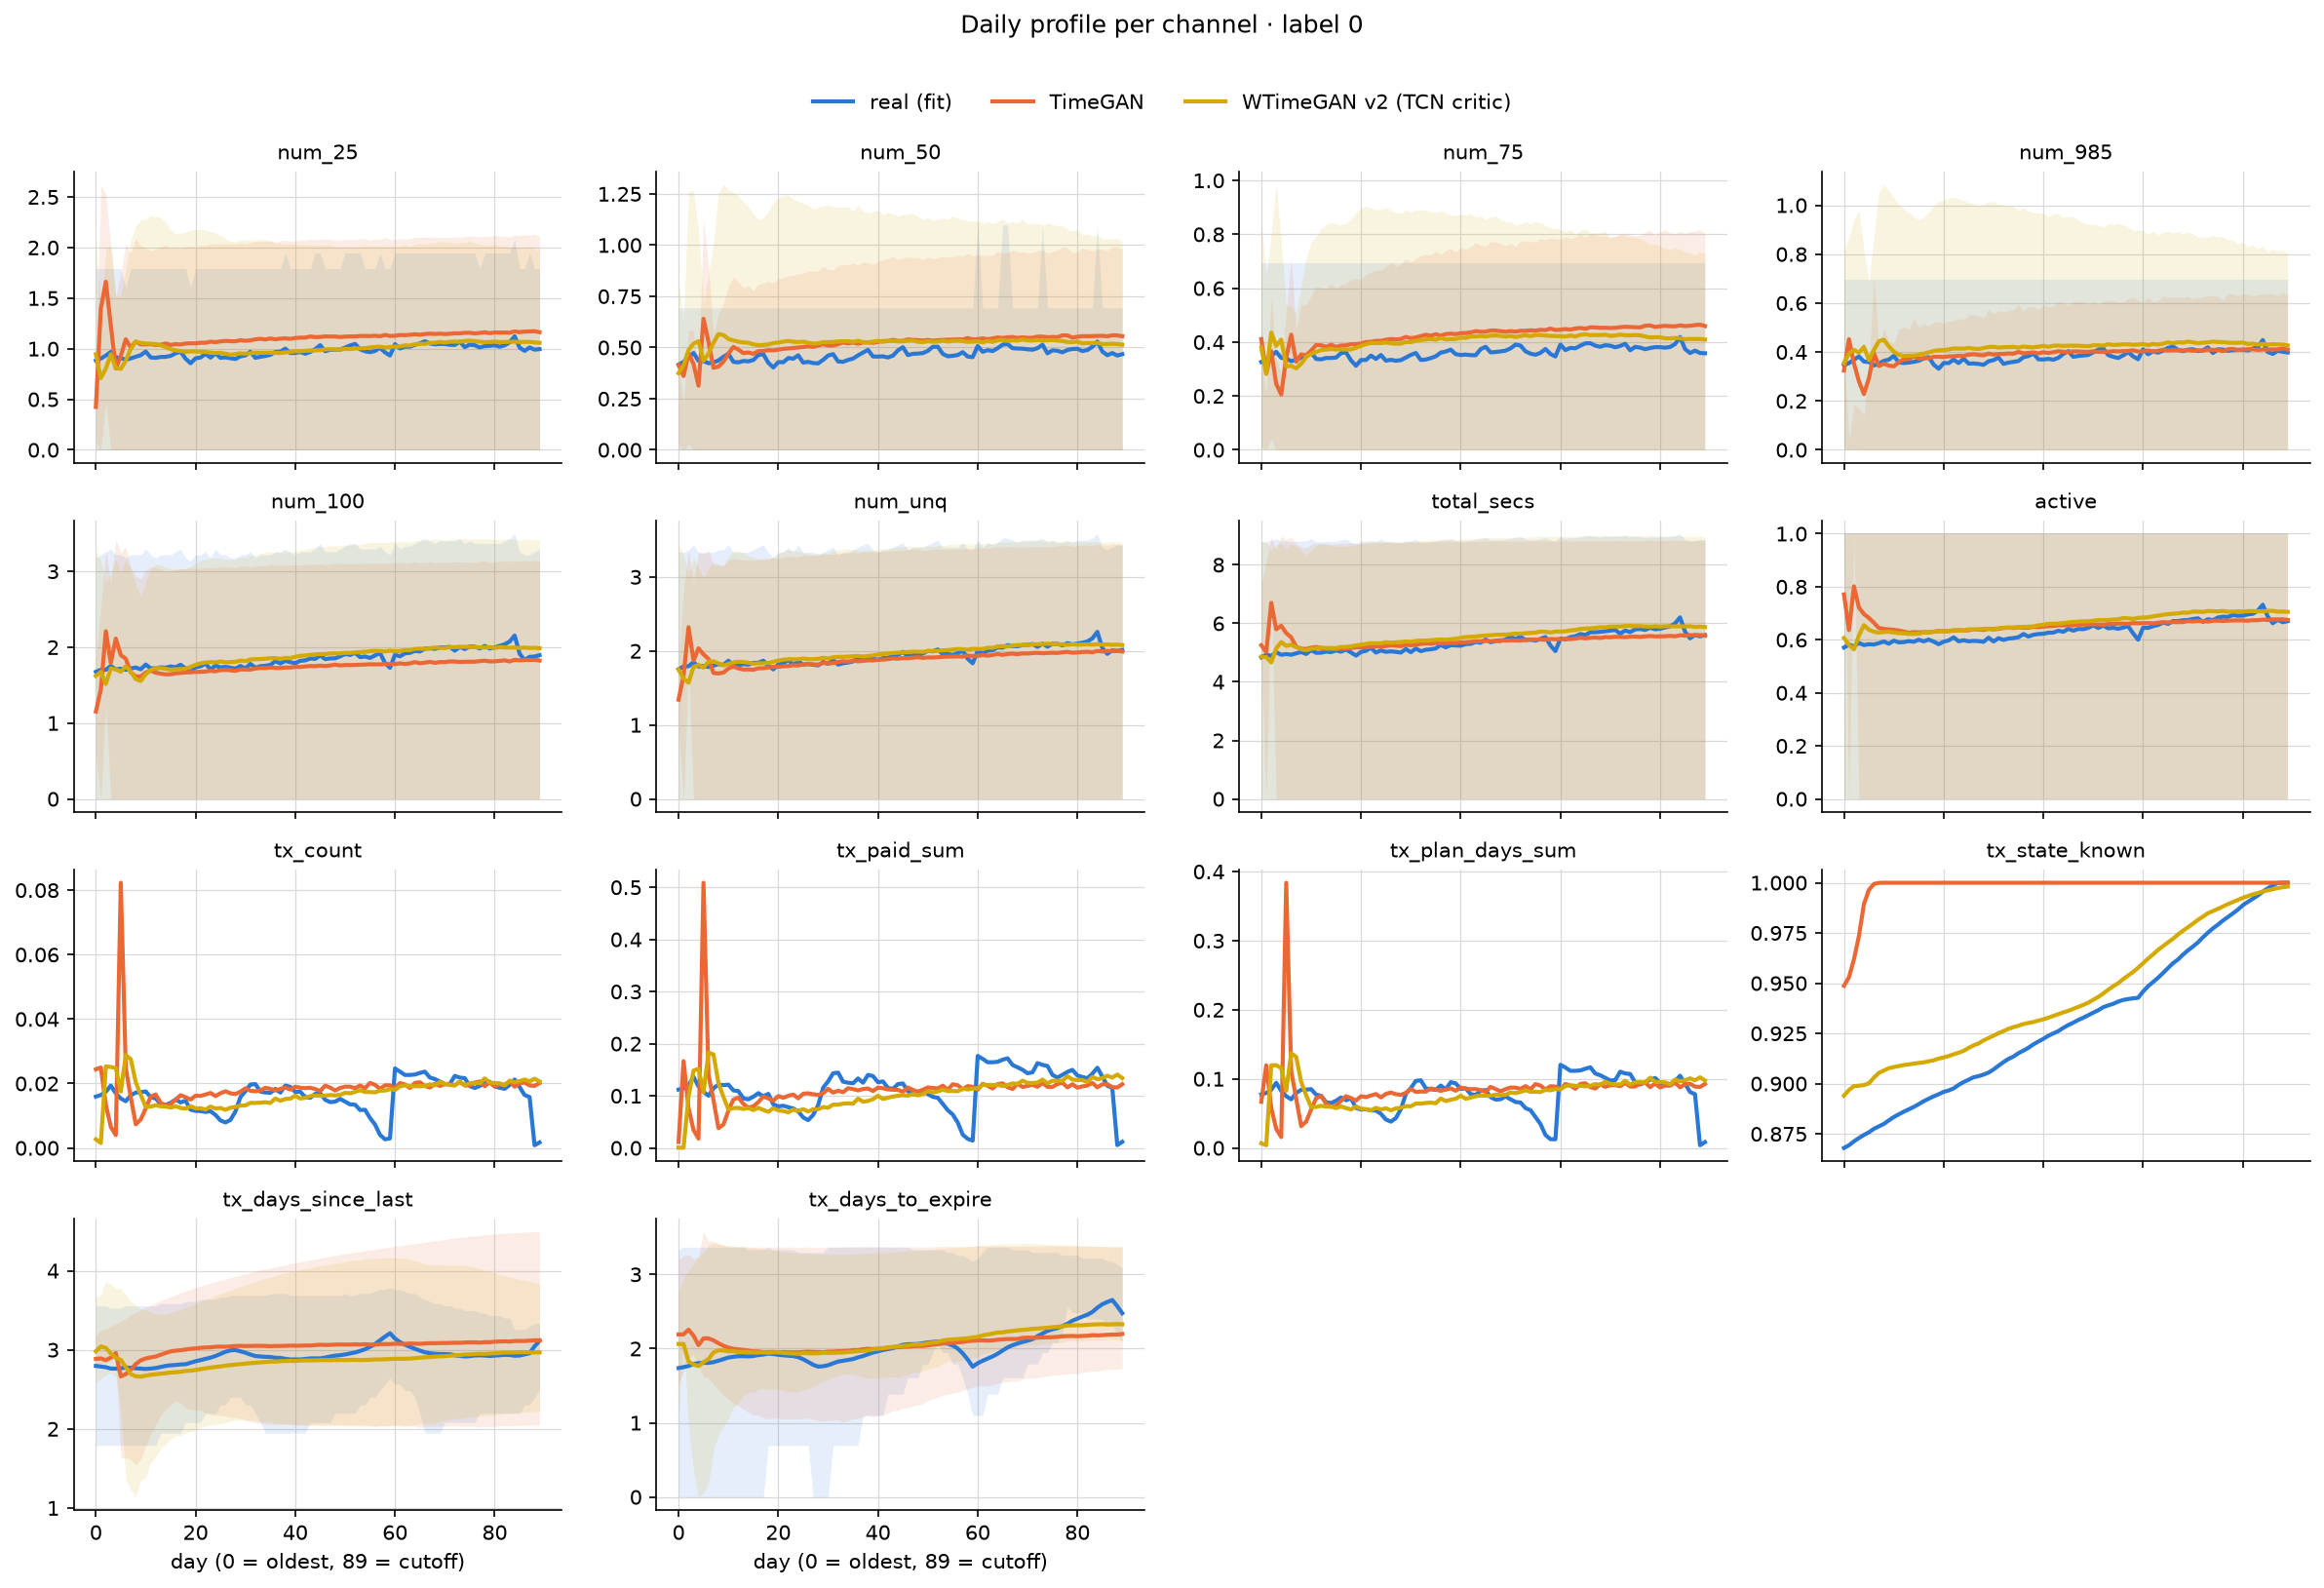
\includegraphics[width=\textwidth]{figures/wgan_tcn/daily_profiles_label0.png}
\caption{Mean and 25 to 75\% band of every channel per day, non-churners.}
\label{fig:w5_profiles0}
\end{figure}

\begin{figure}[H]
\centering
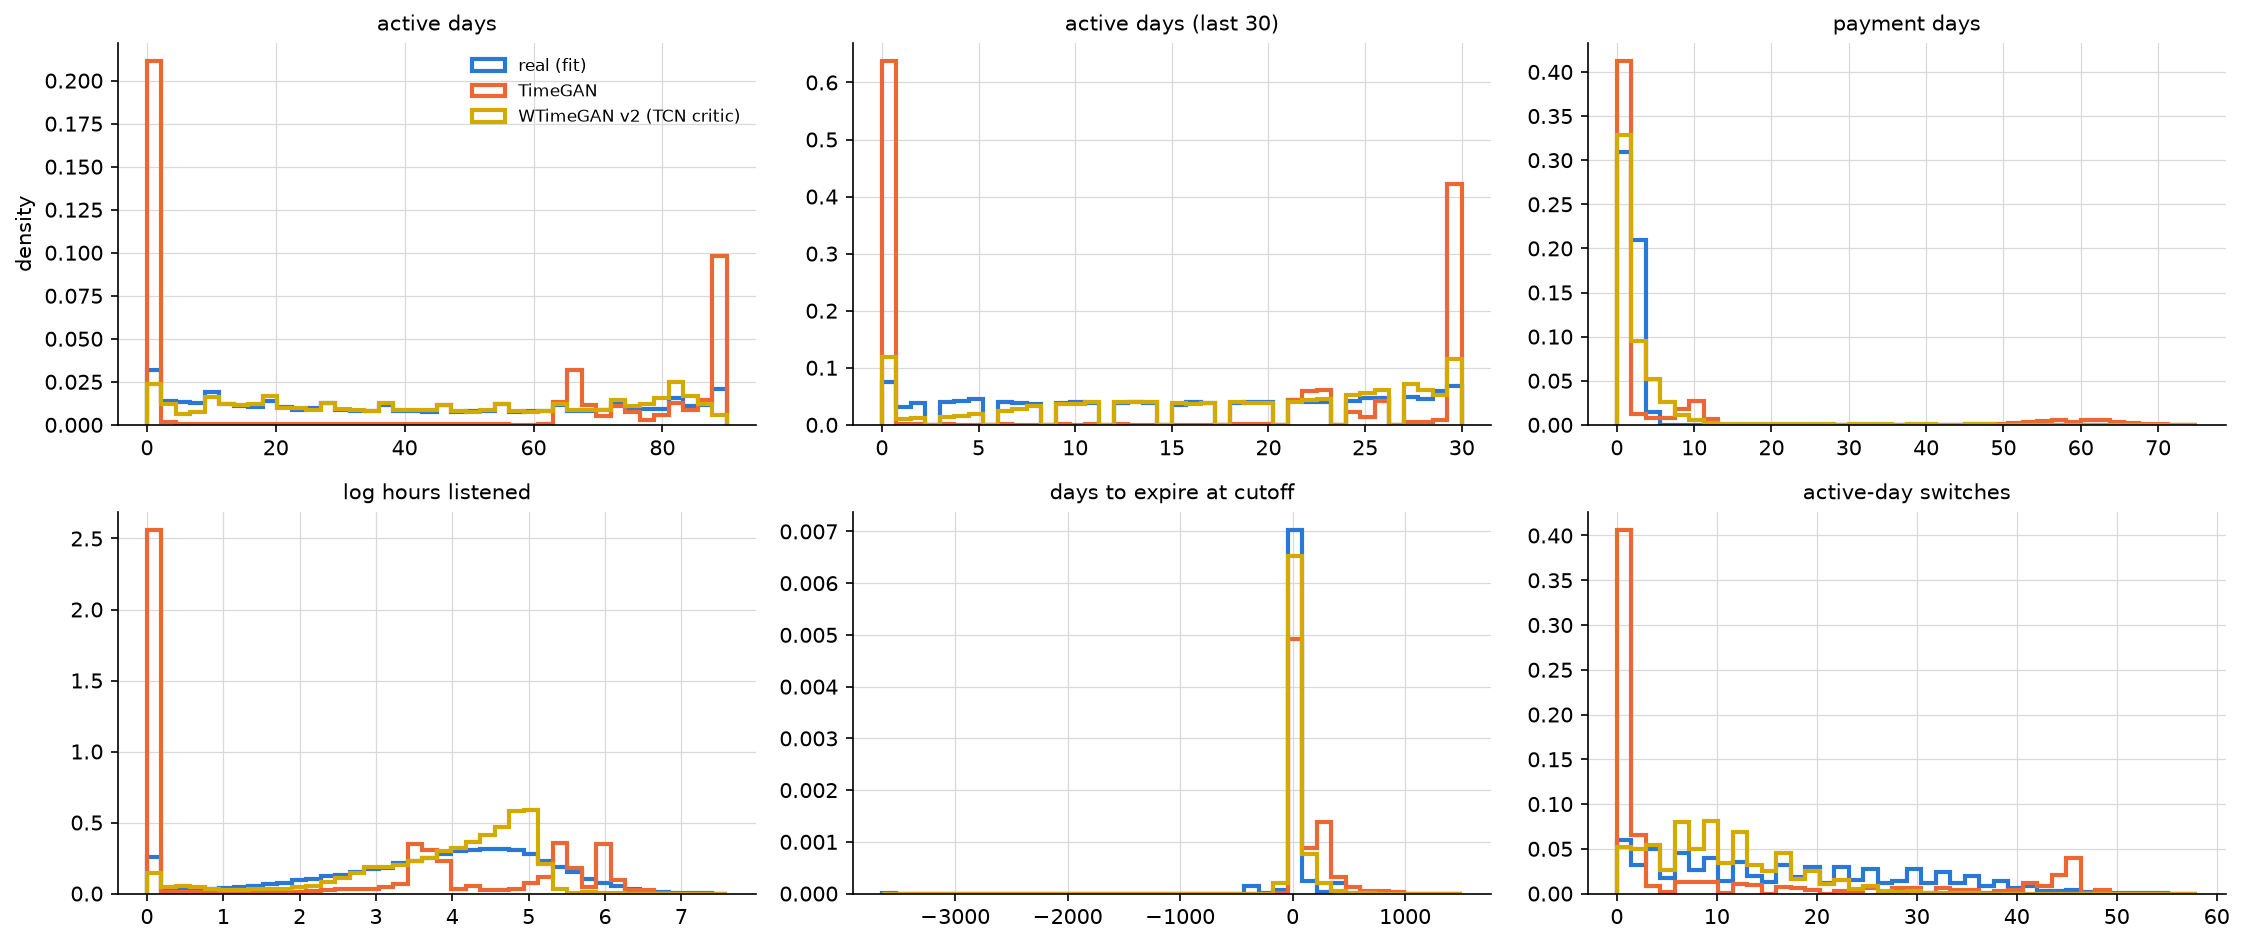
\includegraphics[width=\textwidth]{figures/wgan_tcn/aggregates_label1.png}\\[0.3em]
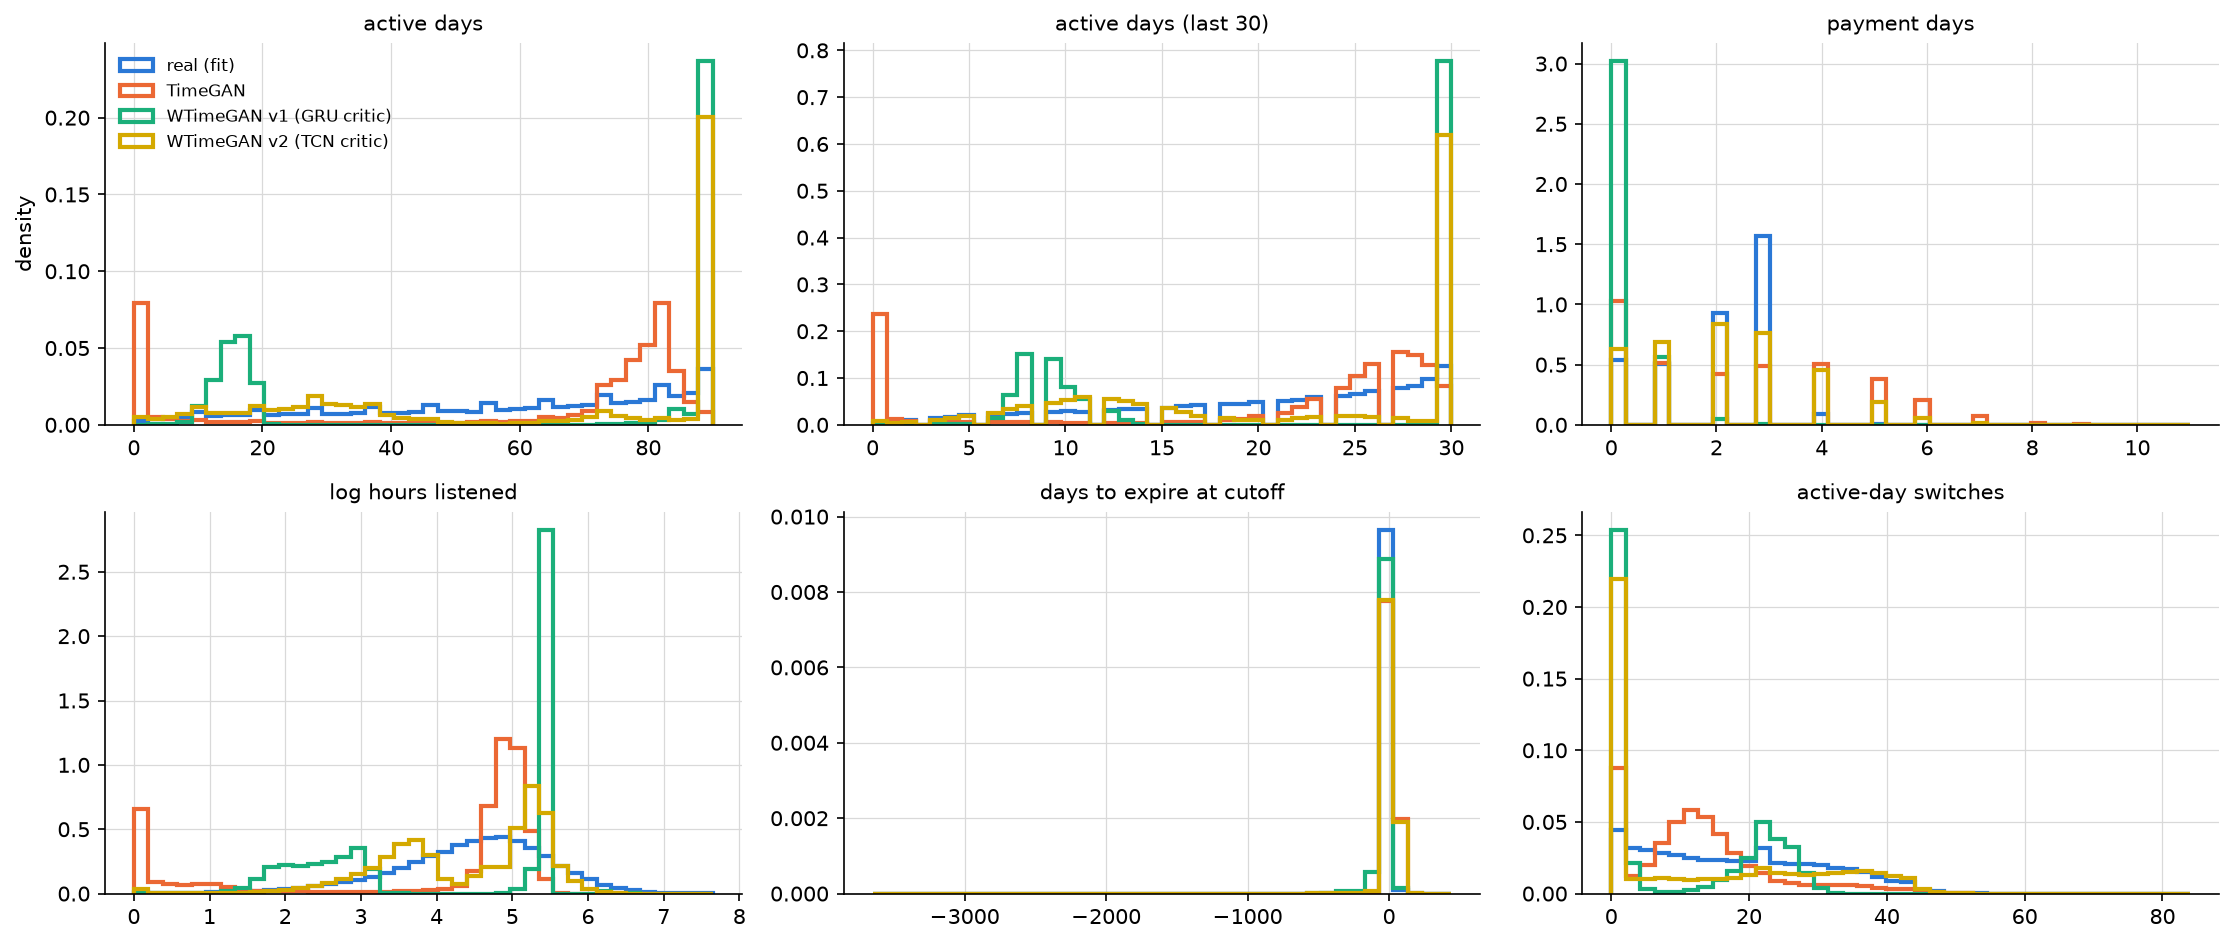
\includegraphics[width=\textwidth]{figures/wgan_tcn/aggregates_label0.png}
\caption{Per-customer aggregates for churners (top) and non-churners (bottom): active days, active days in the last 30, payment days, log hours listened, days to expiry at the cutoff and active-day switches.}
\label{fig:w5_aggregates}
\end{figure}

\paragraph{Individual customers.} Figures~\ref{fig:w5_slices_old} and~\ref{fig:w5_slices} show single customers as heatmaps (rows are days, columns are channels). Real customers alternate active and inactive days and pay a few times. TimeGAN churners are often flat: inactive for the whole window, or active every day. v2 customers have long runs of activity with gaps, realistic listening levels and occasional payments, but fewer on/off switches than real ones.

\begin{figure}[H]
\centering
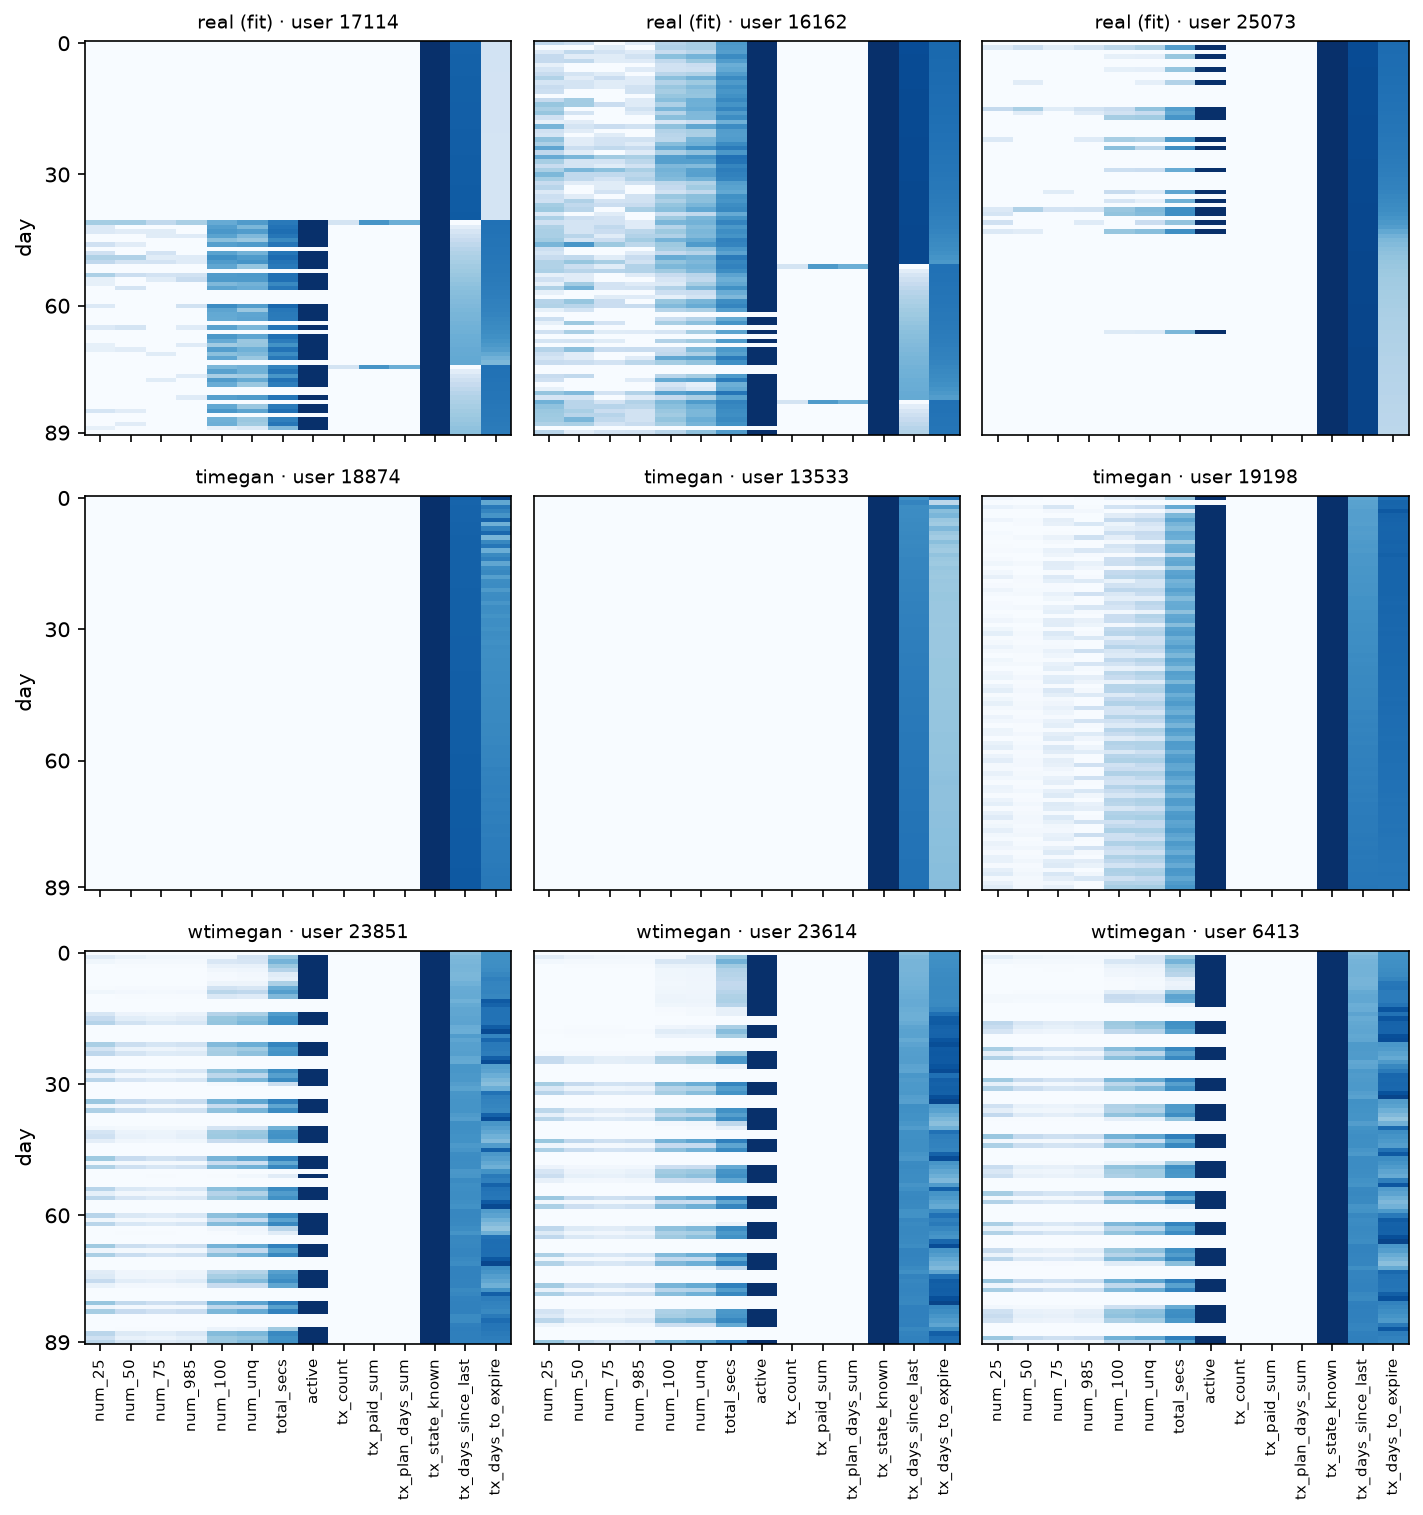
\includegraphics[width=0.85\textwidth]{figures/gan_models/user_slices_label1.png}
\caption{Real, TimeGAN and Wasserstein v1 churners, three customers each.}
\label{fig:w5_slices_old}
\end{figure}

\begin{figure}[H]
\centering
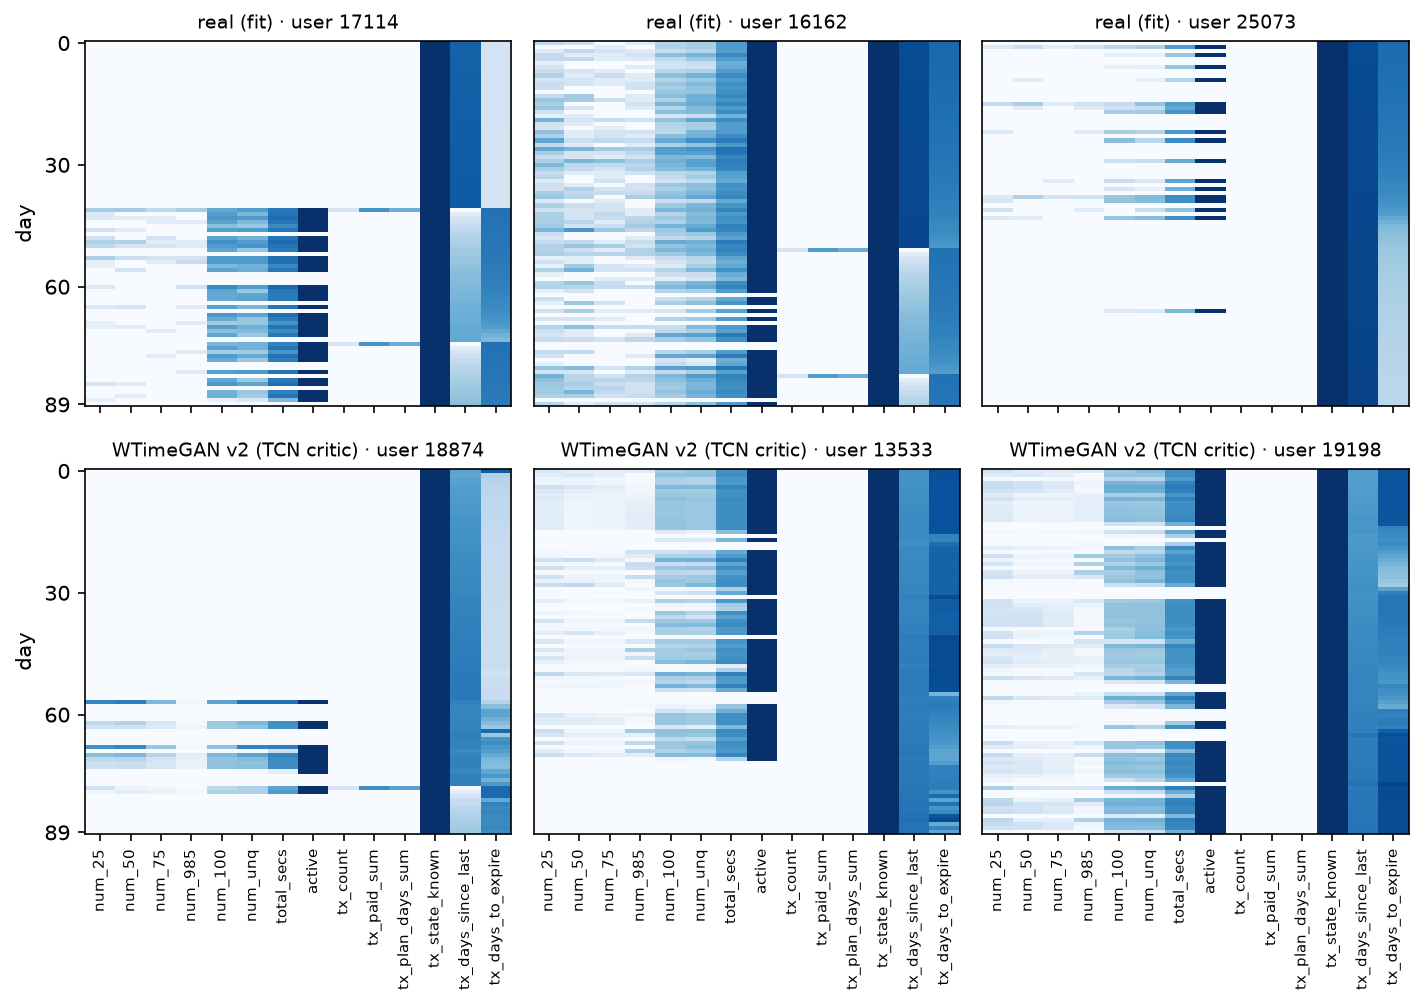
\includegraphics[width=0.85\textwidth]{figures/wgan_tcn/user_slices_label1.png}
\caption{Real and Wasserstein v2 churners, three customers each. The equivalent figures for non-churners are \texttt{figures/gan\_models/user\_slices\_label0.png} and \texttt{figures/wgan\_tcn/user\_slices\_label0.png}.}
\label{fig:w5_slices}
\end{figure}

\subsection{Payment Dynamics}
\label{sec:w5_domain}

The Workshop~2 trajectory model learns when a customer pays from the state channels, and a real manual payer pays around the expiry of the plan. We check whether the generated payments and states follow the same rules (Table~\ref{tab:w5_domain}), with the state as generated and with the state rebuilt from the generated payments.

\begin{table}[H]
\centering
\renewcommand{\arraystretch}{1.3}
\begin{adjustbox}{max width=\textwidth}
\begin{tabular}{|c|l|r|r|r|r|r|}
\hline
\textbf{Class} & \textbf{Source} & \textbf{Pay days} & \textbf{Countdown} & \textbf{Reset} & \textbf{Near expiry (gen.)} & \textbf{Near expiry (rebuilt)} \\ \hline
\multirow{4}{*}{Churners} & Real \texttt{fit} & 1.55\% & 100\% & 93\% & \multicolumn{2}{c|}{40\%} \\ \cline{2-7}
 & TimeGAN & 6.45\% & 59\% & 21\% & 1.0\% & 0.3\% \\ \cline{2-7}
 & Wasserstein v1 & 0.19\% & 38\% & 14\% & 33\% & 5.6\% \\ \cline{2-7}
 & Wasserstein v2 & 2.57\% & 51\% & 5\% & 26\% & 5.5\% \\ \hline
\multirow{4}{*}{Non-churners} & Real \texttt{fit} & 2.28\% & 100\% & 97\% & \multicolumn{2}{c|}{58\%} \\ \cline{2-7}
 & TimeGAN & 2.65\% & 47\% & 13\% & 22\% & 11\% \\ \cline{2-7}
 & Wasserstein v1 & 0.20\% & 48\% & 4\% & 31\% & 9.0\% \\ \cline{2-7}
 & Wasserstein v2 & 2.42\% & 49\% & 26\% & 16\% & 9.6\% \\ \hline
\end{tabular}
\end{adjustbox}
\caption{Payment dynamics. Pay days: share of days with a payment. Countdown: share of days without payment where \texttt{tx\_days\_to\_expire} drops by one. Reset: share of payment days where the expiry jumps by the purchased plan days. Near expiry: share of payments made within 3 days of the expiry known the day before, with the generated state and with the state rebuilt from the generated payments.}
\label{tab:w5_domain}
\end{table}

v2 generates payments at a plausible rate and amount (2.6\,\% of the days for churners, 27 plan days and 98\,NTD per payment against 41 days and 201\,NTD for real churners; TimeGAN gives 10 days and 20\,NTD). It does not learn when to pay. Its generated expiry counts down correctly on half of the days and resets on 5\,\% of the payment days, against 100\,\% and 93\,\% for real customers. With the state rebuilt from its own payments, only 5.5\,\% of its payments fall within 3 days of the expiry, against 40\,\% for real churners: v2 places payments at days that are nearly unrelated to the plan expiry. Figure~\ref{fig:w5_pay_expiry} shows the same problem for TimeGAN and v1, whose payment rates stay flat around the expiry, where real customers have a clear peak just after it.

\begin{figure}[H]
\centering
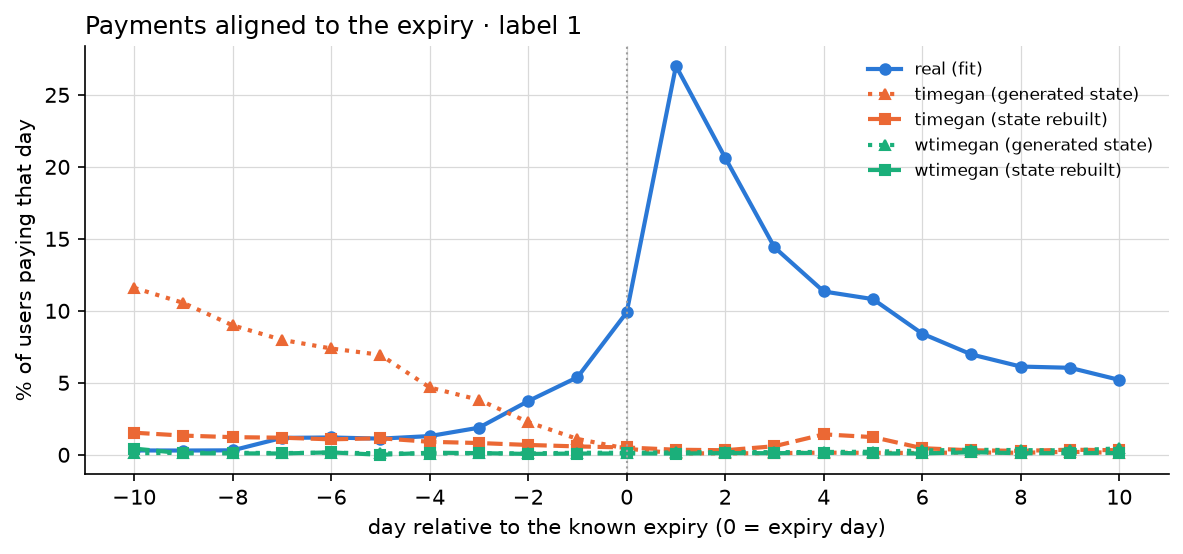
\includegraphics[width=0.85\textwidth]{figures/gan_models/pay_by_expiry_label1.png}
\caption{Share of churners paying on each day relative to their known expiry. Real customers renew in the days right after the expiry; TimeGAN and v1 show no peak after it. The figure for non-churners is \texttt{figures/gan\_models/pay\_by\_expiry\_label0.png}.}
\label{fig:w5_pay_expiry}
\end{figure}

\subsection{Best Seeds of the Tuned Models}
\label{sec:w5_best_seeds}

The figures above come from the single hand-set run. To see what the tuned models of Section~\ref{sec:w5_robustness} generate, we took for each GAN and class the seed with the lowest Fréchet distance out of five: TimeGAN seed 3 (0.344) and v2 seed 0 (0.117) for churners, TimeGAN seed 0 (0.149) and v2 seed 2 (0.058) for non-churners. These are the best cases, chosen on the test metric itself, so they show what each model can reach, not what it typically gives; the typical values are the means of Table~\ref{tab:w5_seeds}. The figures are produced by \path{workshops/w5/plot_seed_runs.py}.

\begin{figure}[H]
\centering
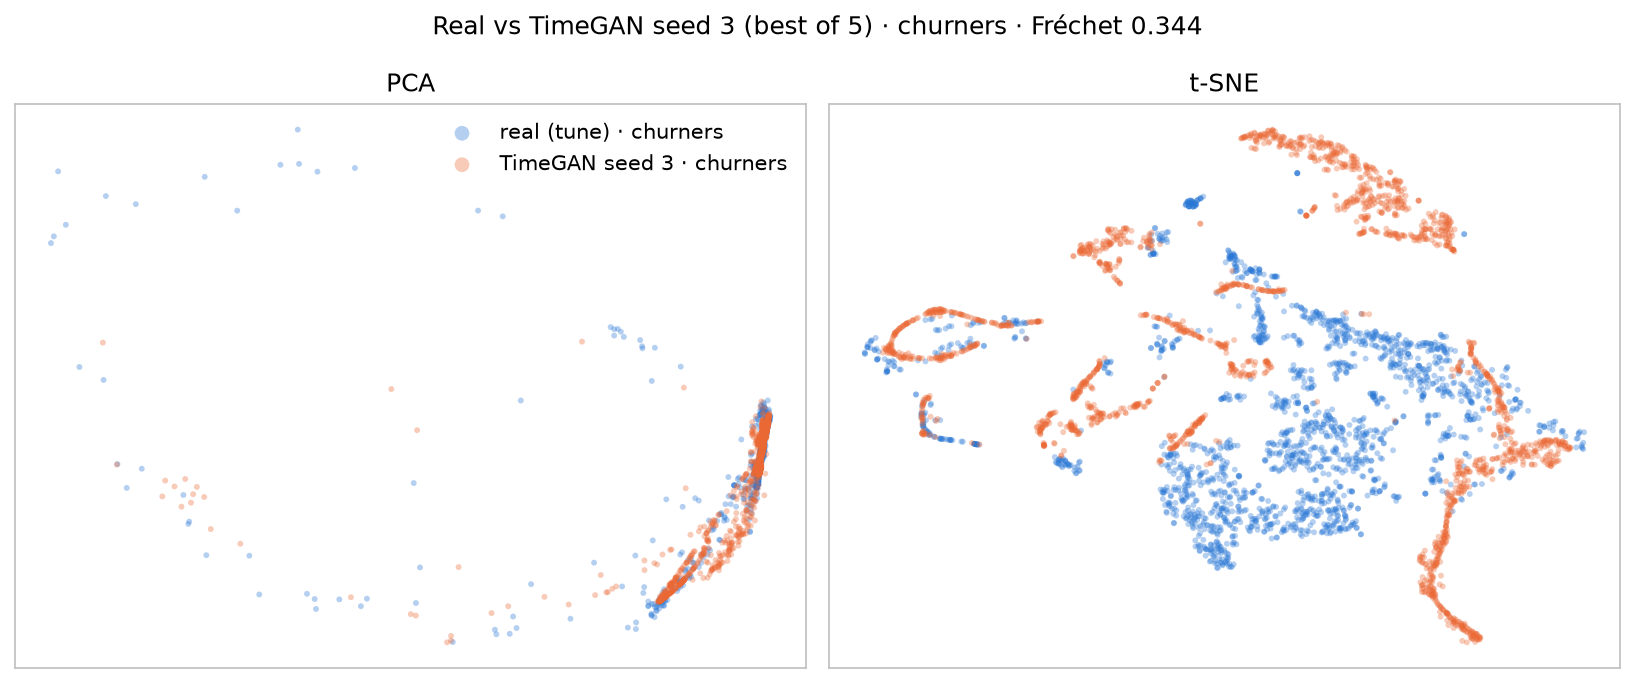
\includegraphics[width=0.92\textwidth]{figures/experiments/embedding_label1_timegan.png}\\[0.3em]
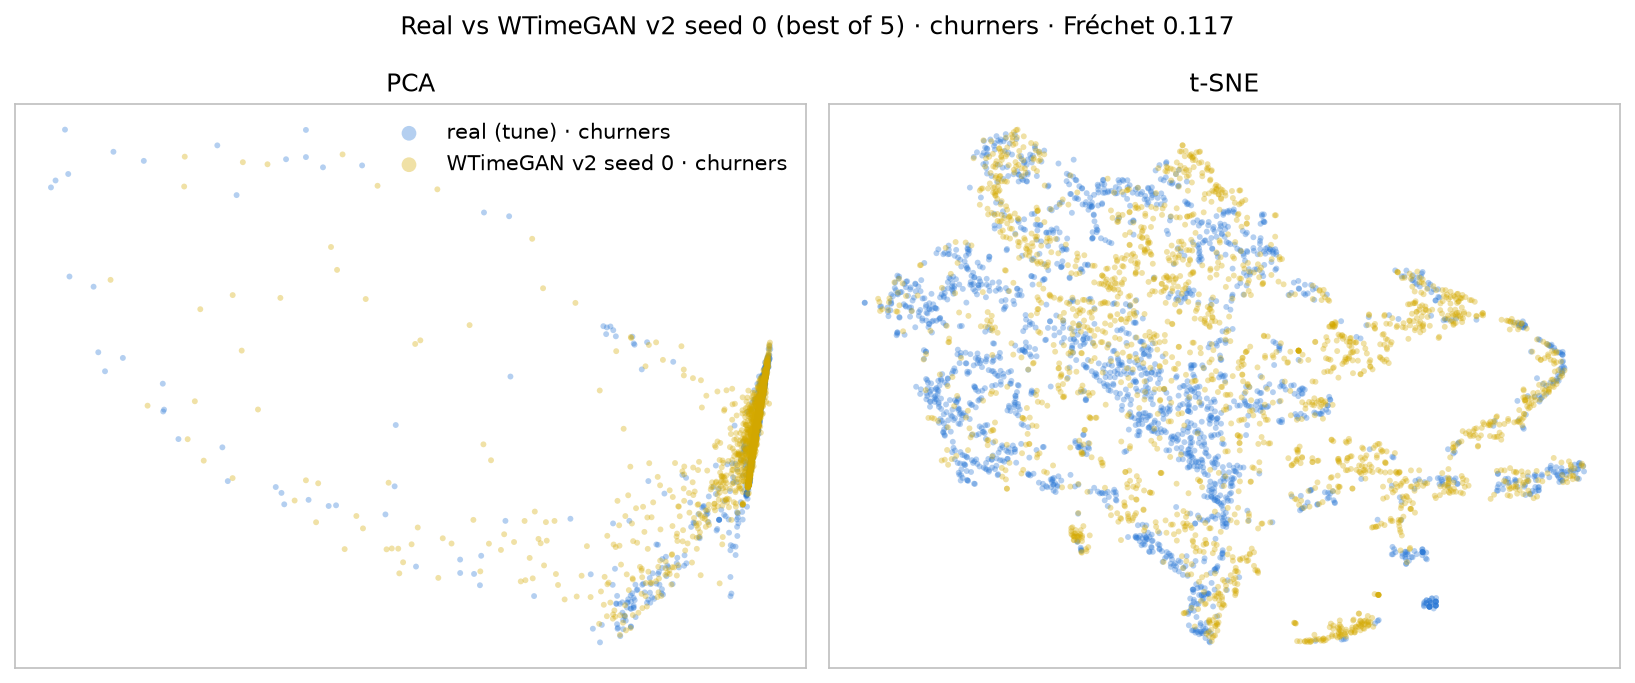
\includegraphics[width=0.92\textwidth]{figures/experiments/embedding_label1_wtimegan_tcn.png}
\caption{Churners, best seed of each tuned GAN: PCA and t-SNE of the Workshop~2 LSTM features, real \texttt{tune} against synthetic.}
\label{fig:w5_best_emb_1}
\end{figure}

\begin{figure}[H]
\centering
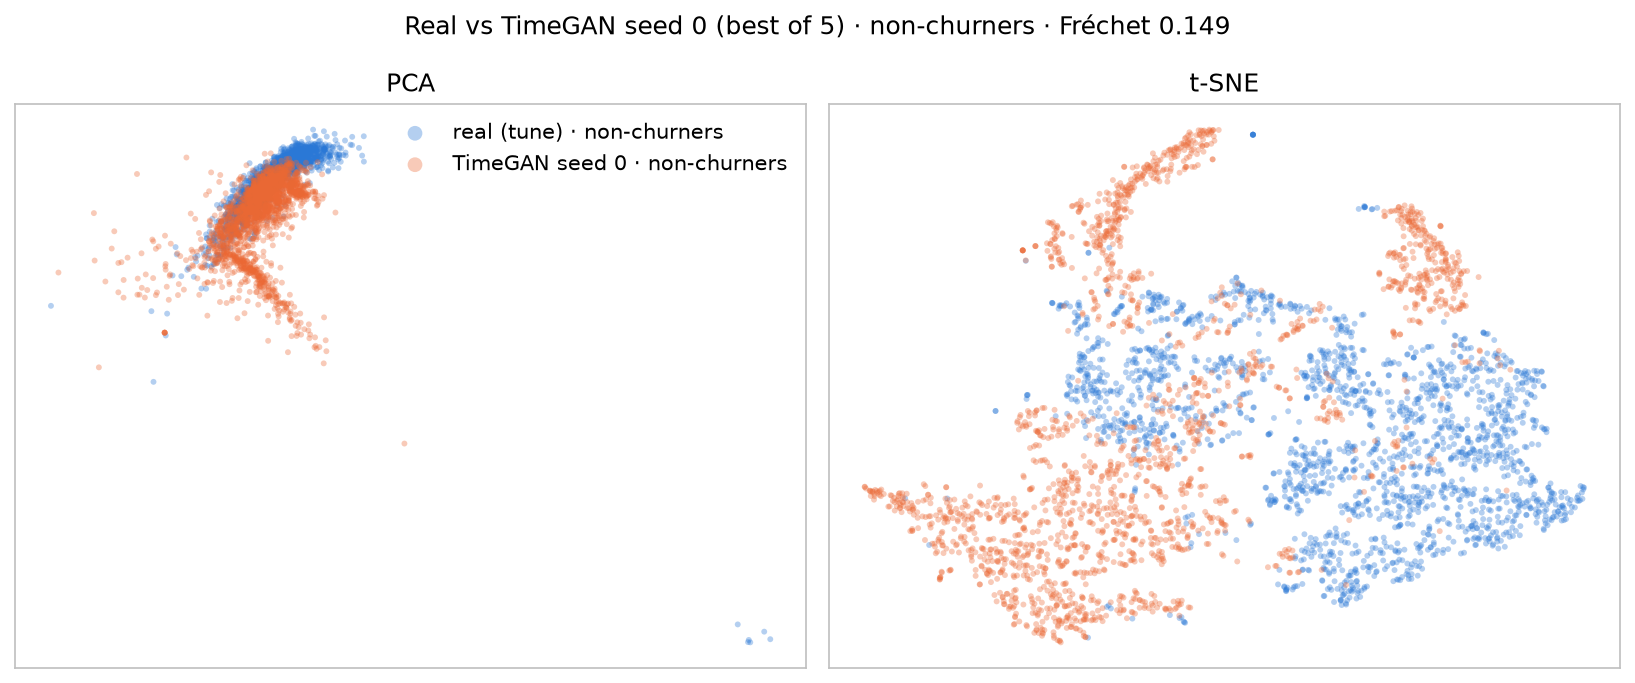
\includegraphics[width=0.92\textwidth]{figures/experiments/embedding_label0_timegan.png}\\[0.3em]
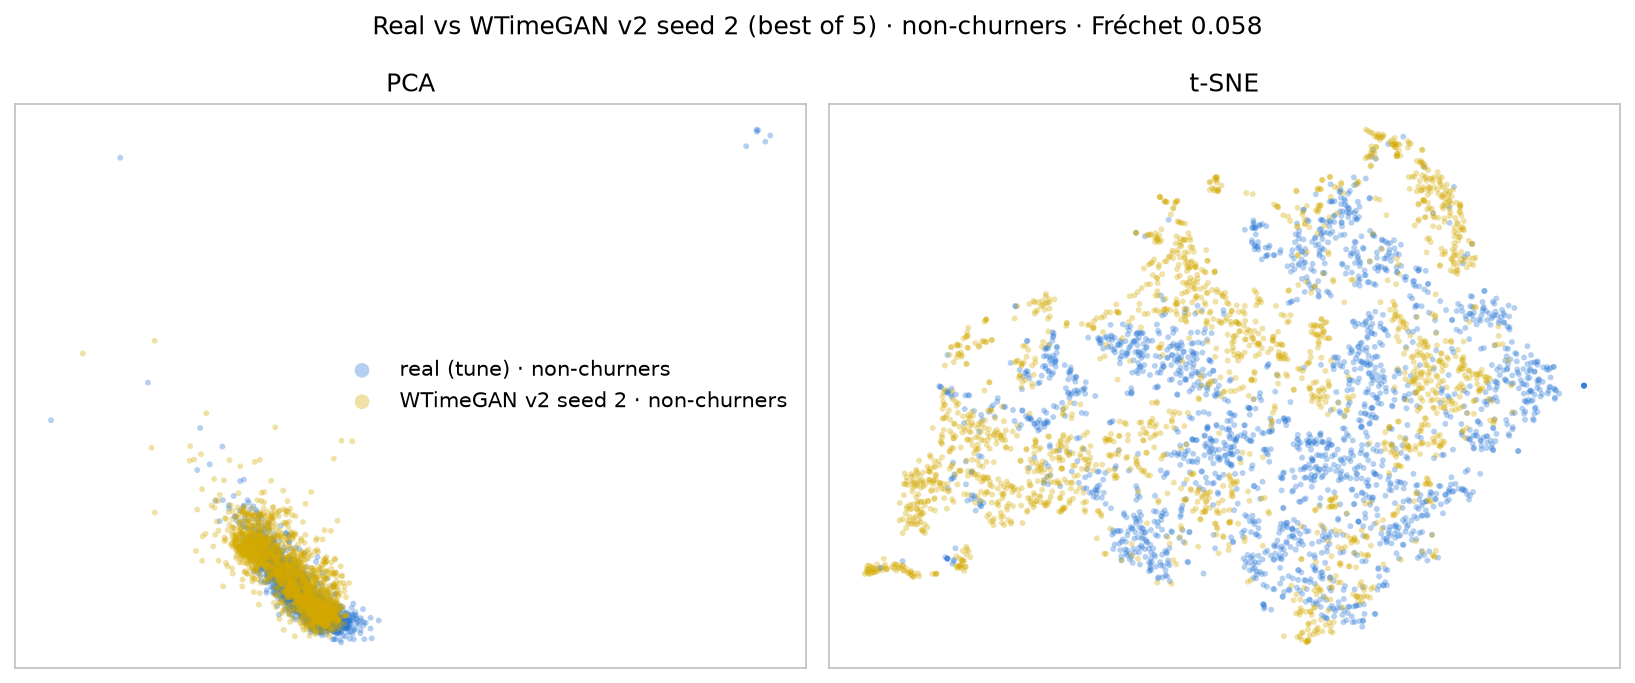
\includegraphics[width=0.92\textwidth]{figures/experiments/embedding_label0_wtimegan_tcn.png}
\caption{Non-churners, best seed of each tuned GAN.}
\label{fig:w5_best_emb_0}
\end{figure}

The best seeds keep the ranking of the single run. v2 customers mix with real ones over the whole t-SNE map in both classes. The best TimeGAN churners no longer collapse into one curve, as the hand-set run did, but they still form several thin curves at the edges of the real cloud, and the best TimeGAN non-churners cover one half of the map while real customers occupy the other.

\begin{figure}[H]
\centering
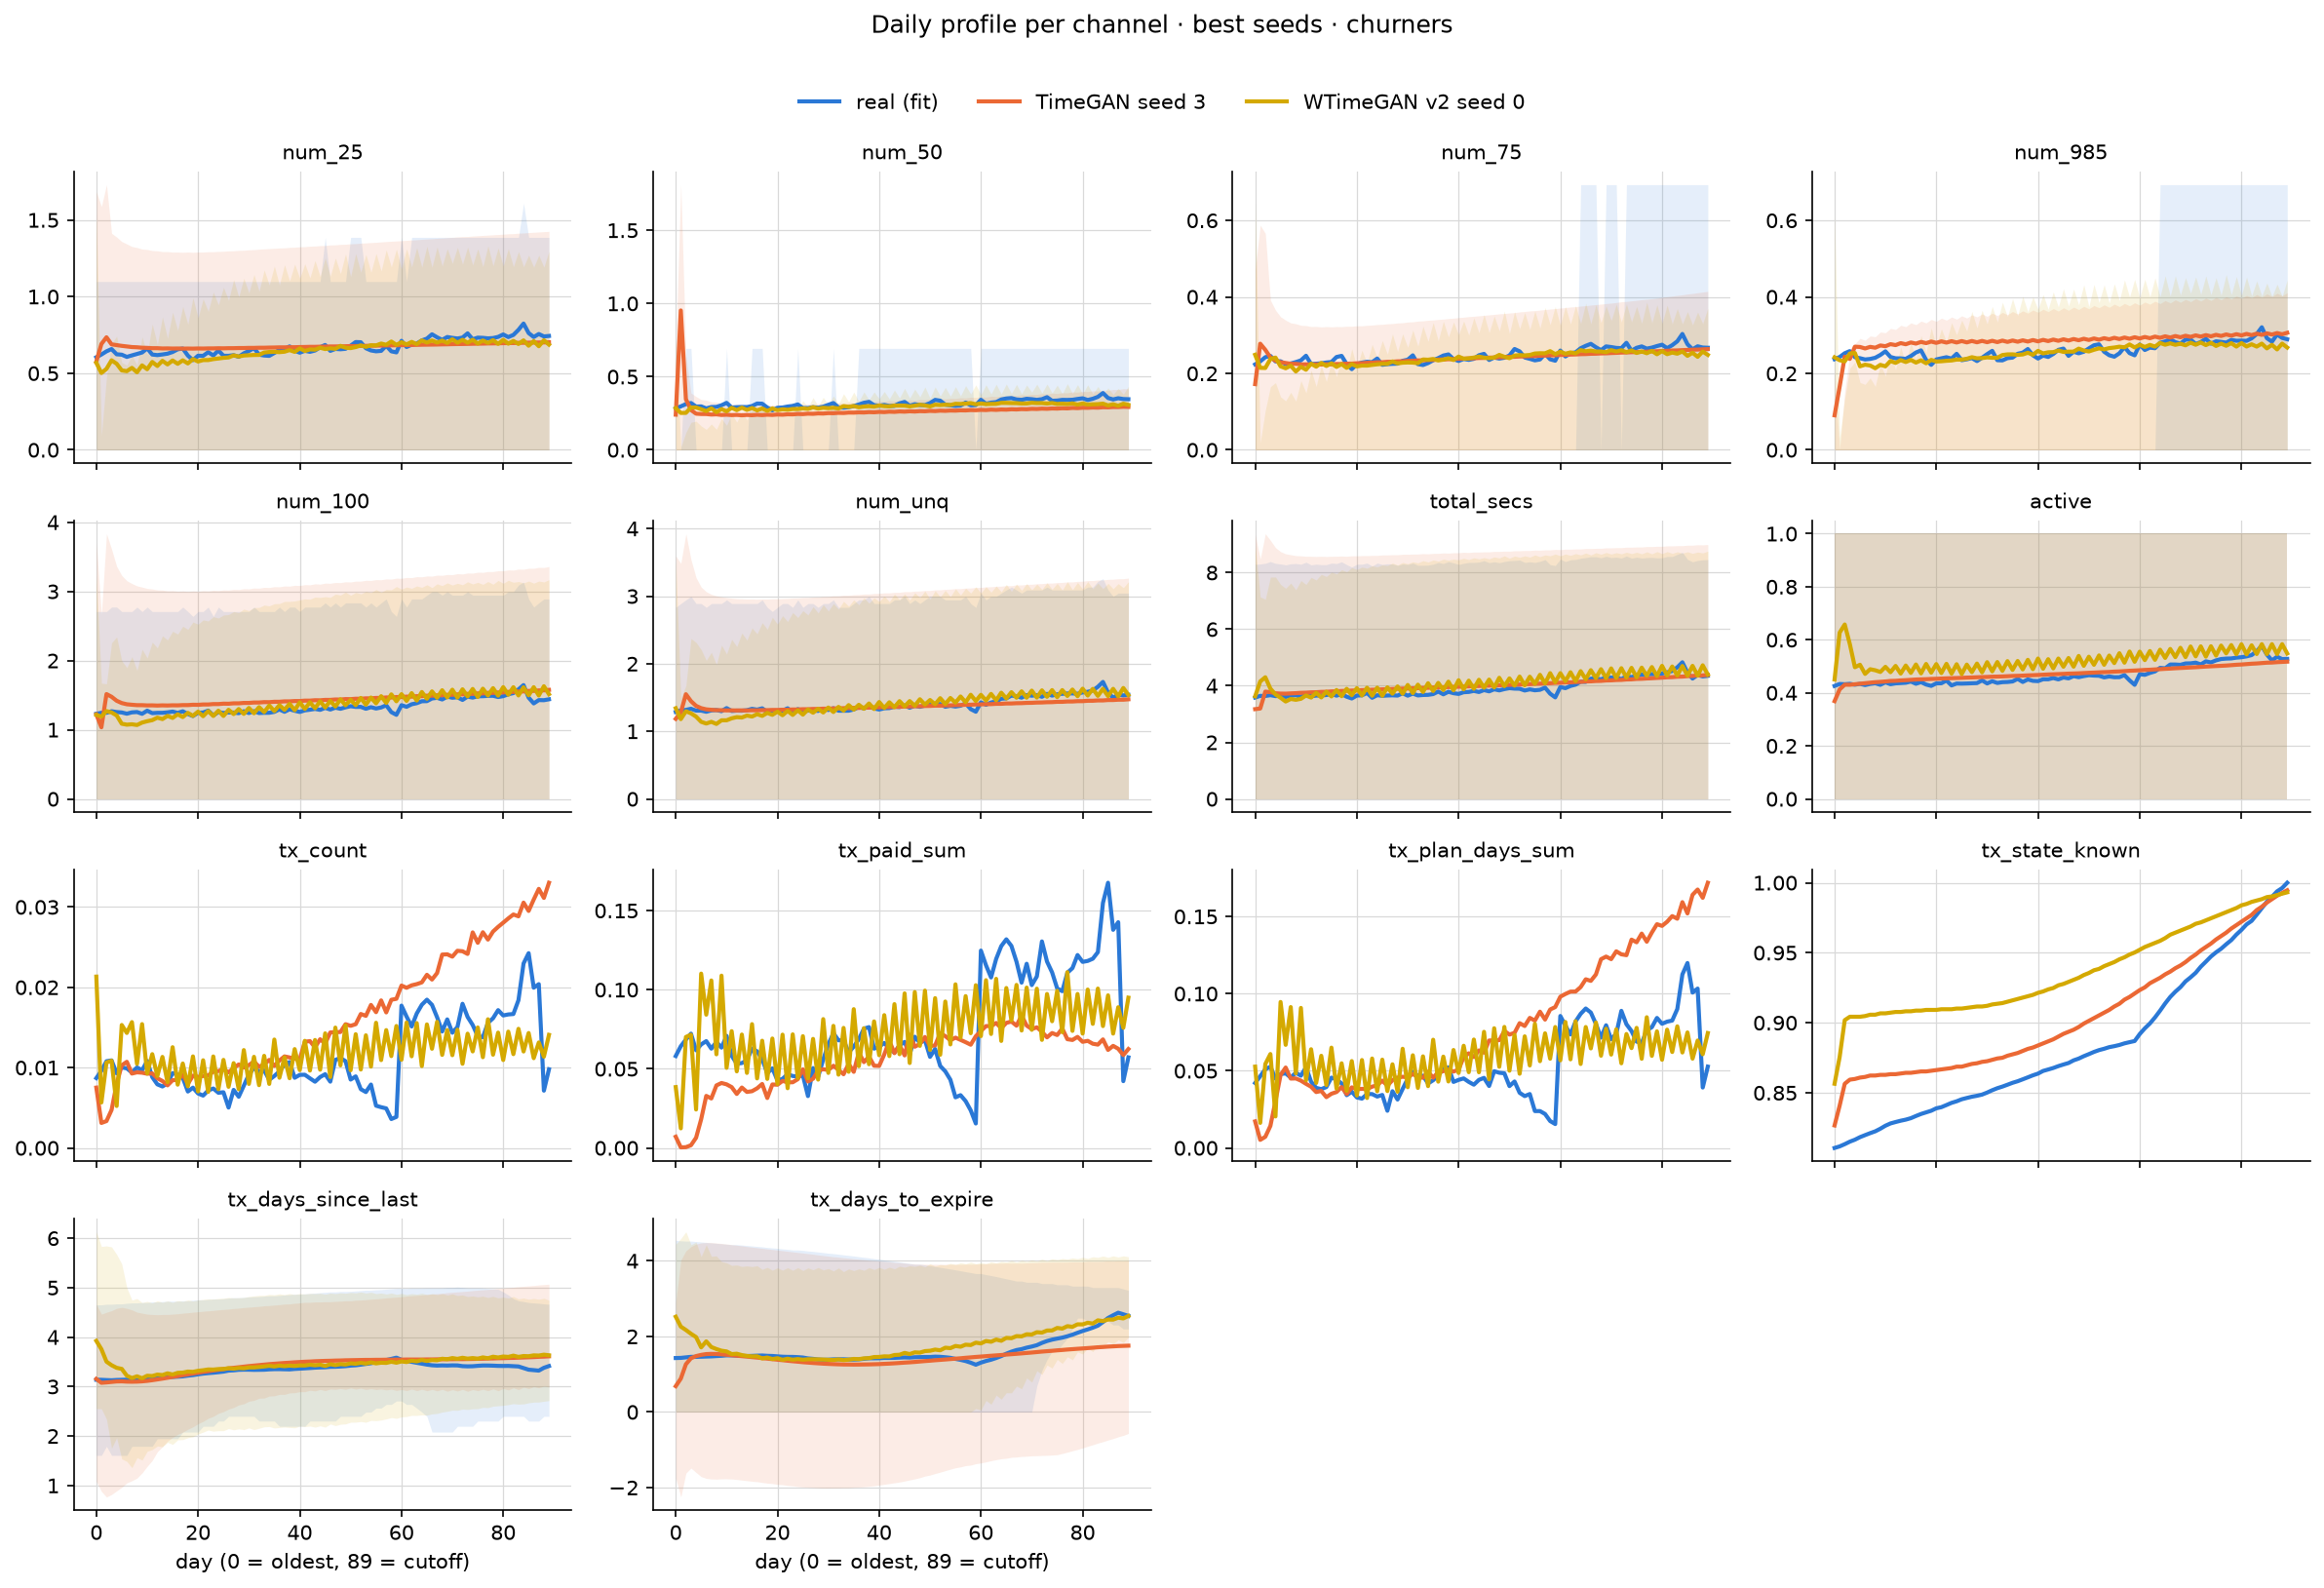
\includegraphics[width=\textwidth]{figures/experiments/daily_profiles_label1.png}
\caption{Churners, best seeds: mean of each channel per day (line) and 25--75\,\% band.}
\label{fig:w5_best_profiles_1}
\end{figure}

\begin{figure}[H]
\centering
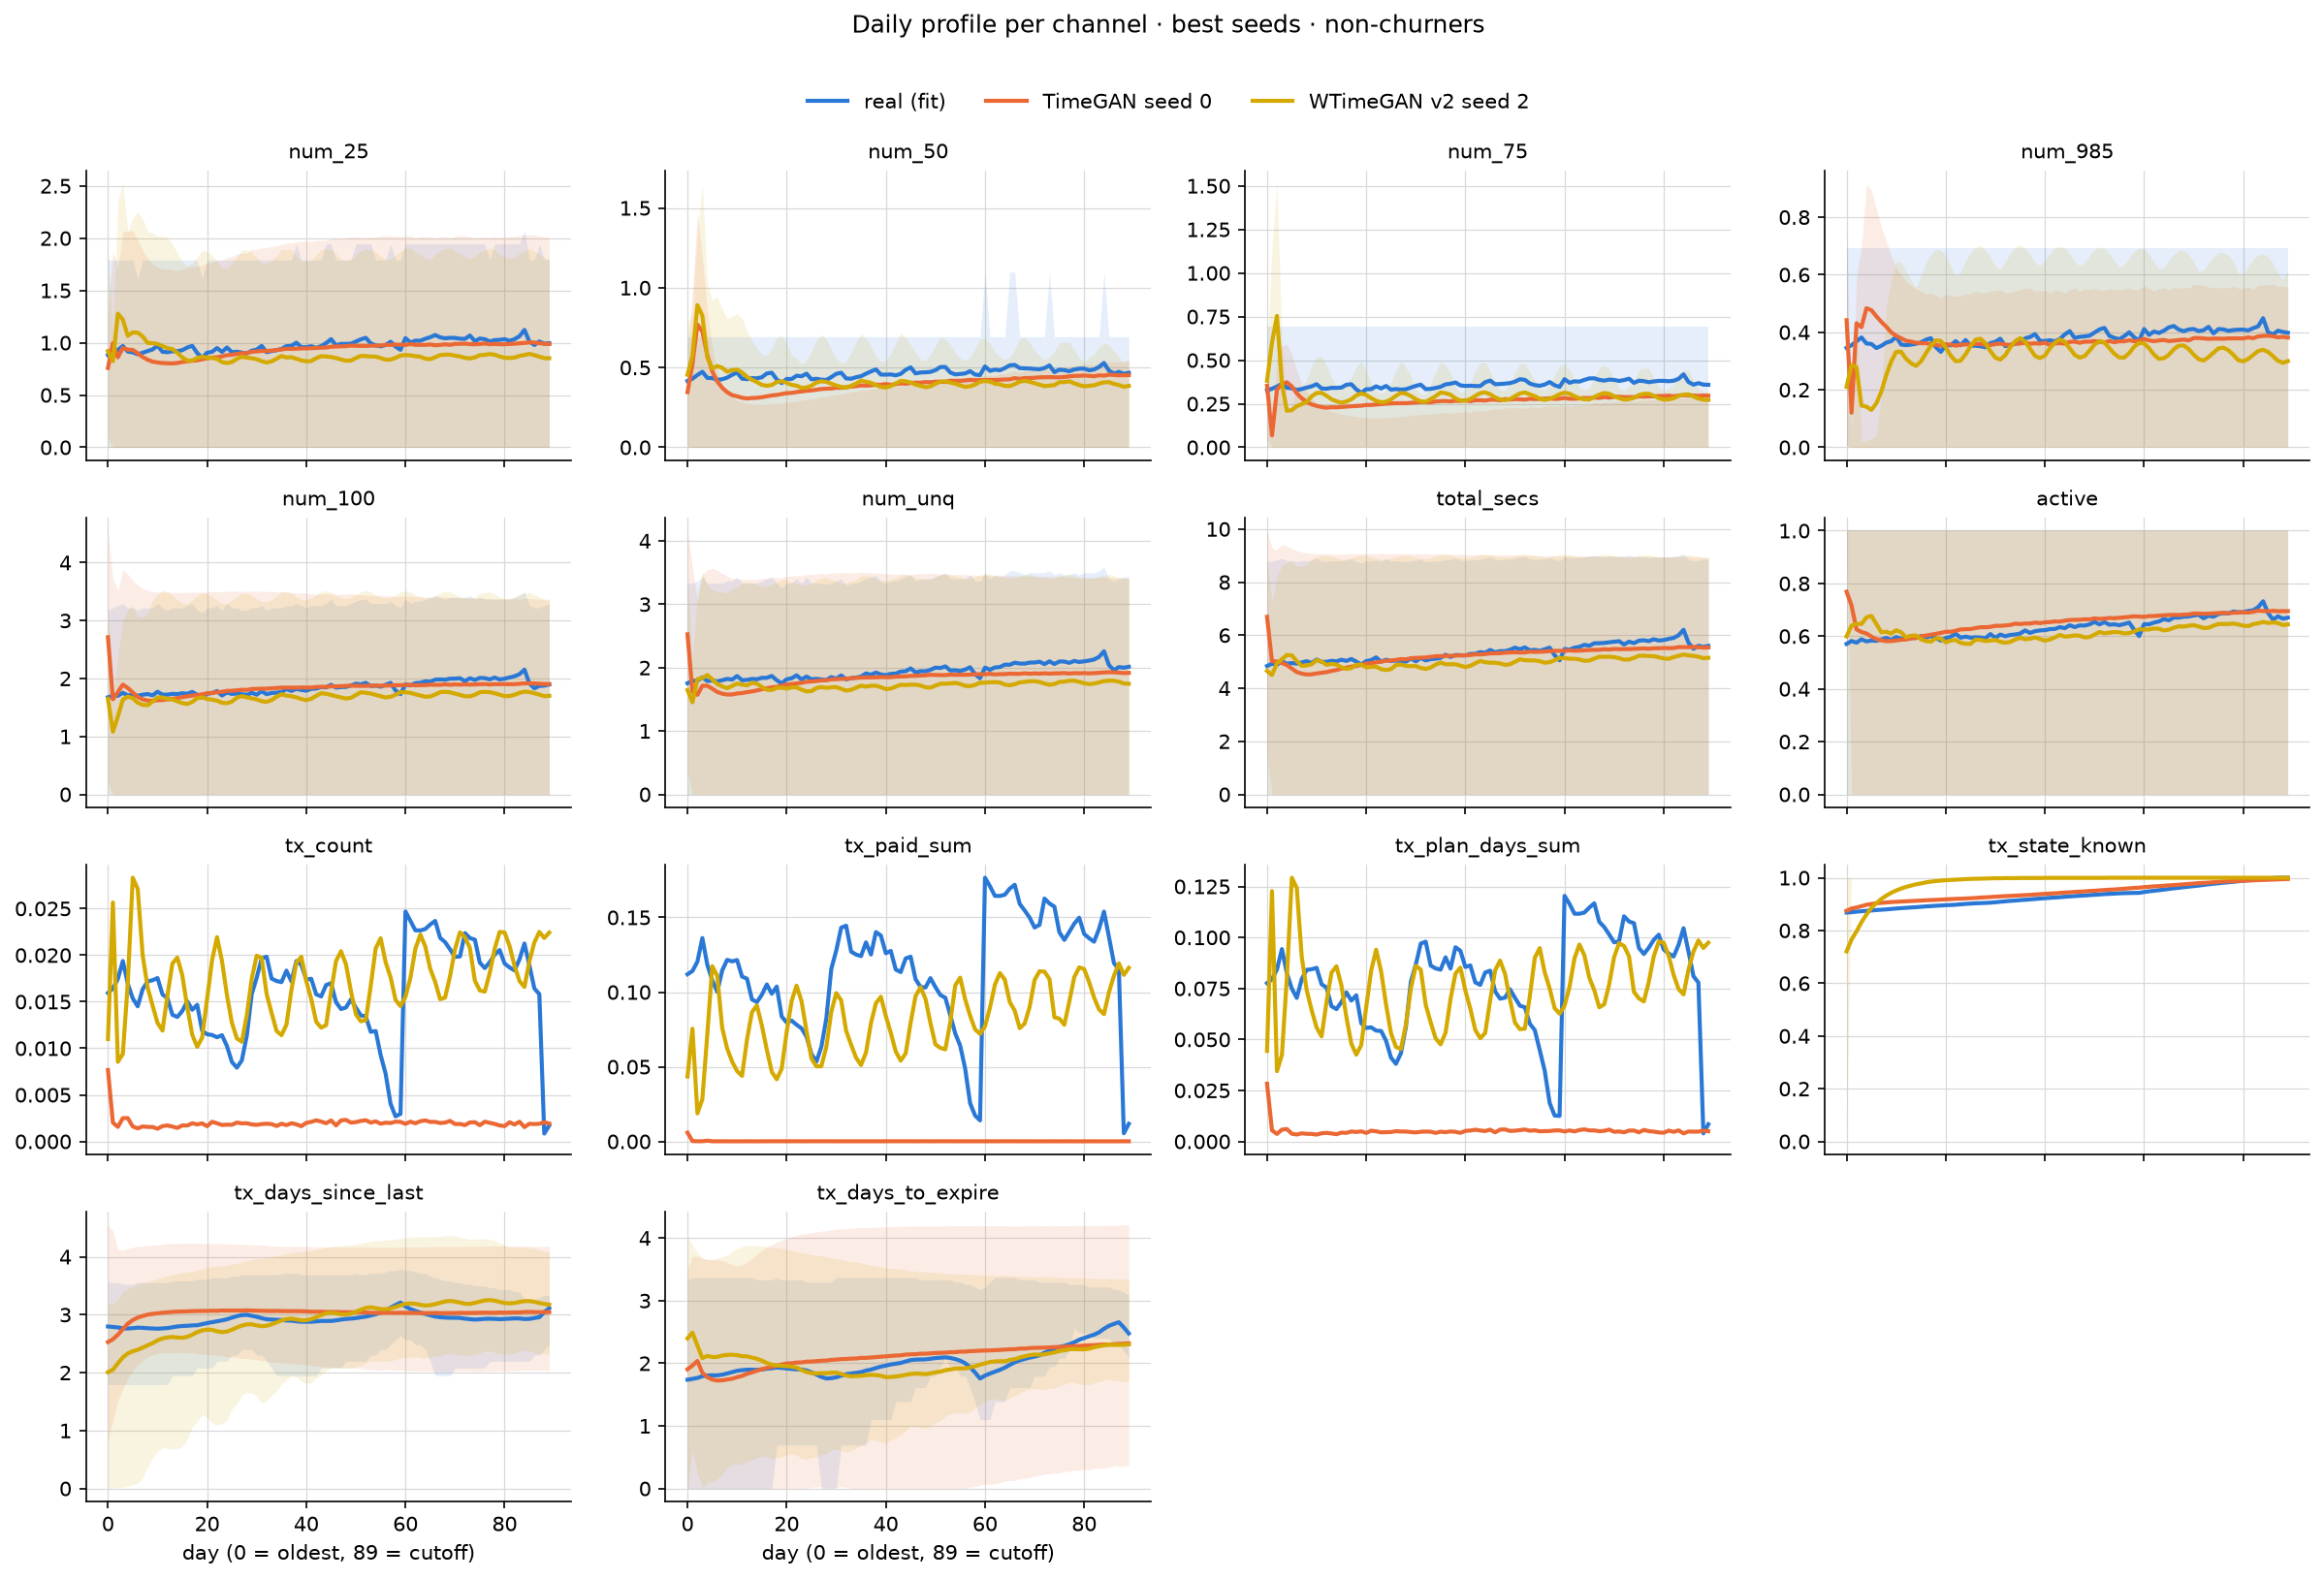
\includegraphics[width=\textwidth]{figures/experiments/daily_profiles_label0.png}
\caption{Non-churners, best seeds.}
\label{fig:w5_best_profiles_0}
\end{figure}

In the listening channels both GANs follow the real daily means closely. The payment channels show the weaknesses of Section~\ref{sec:w5_domain} in a different form. The best TimeGAN non-churners almost never pay: their daily share of payments stays near 0.002 against about 0.015 for real non-churners, and their paid amount is close to zero. The best TimeGAN churners pay more and more towards the cutoff in a smooth ramp that real churners do not show. v2 keeps payments at a realistic level but adds a regular oscillation that real customers do not have, with a period of about two days for churners and about a week for non-churners, and it does not reproduce the sharp drops and jumps of the real payment curves around day 60. The tuning therefore improved the overall distance but did not fix the payment dynamics.

% ─────────────────────────────────────────────
\section{Failure Mode Analysis}
\label{sec:w5_failures}
% ─────────────────────────────────────────────

\paragraph{Mode collapse in TimeGAN.} The TimeGAN churners collapsed. Synthetic churners are about 35 times closer to each other than real ones (nearest-neighbour distance 0.16 against 5.57), 46\,\% never listen and 27\,\% listen every day, and the median churner never switches between active and inactive. In the t-SNE projection these customers form a single long curve: the generator maps the noise to a thin line of almost identical sequences. These customers are caricatures of churners, which explains the mean churn probability of 0.75. The non-churners did not collapse (their diversity is close to the real one), but they are polarised as well (5.4\,\% with no active day against 0.2\,\%). Churners are the harder class: half as many training examples (26{,}947 against 56{,}867) and more heterogeneous behaviour (active days from 4 to 83 between the 10th and 90th percentiles).

We ruled out data problems first. The real \texttt{fit} and \texttt{tune} customers have the same distribution (active days at the 10th, 50th and 90th percentiles: 4, 40 and 83 against 4, 38 and 83), the loader rejects missing values, and outliers do not compress the min-max scale.

\paragraph{The discriminator overpowers the generator.} The joint-phase losses of TimeGAN (Table~\ref{tab:w5_timegan_dyn}) show the cross-entropy discriminator winning: its loss falls to 0.2 to 0.6 while the generator loss rises to 3 to 6. A confident discriminator labels every synthetic customer ``fake'' without saying how far it is from the real data, so the generator gets a weak, nearly flat signal and stays where it already deceives the discriminator a little. Nothing in the cross-entropy penalises the customer types that are missing. The Wasserstein loss addresses both points.

\paragraph{Cost of the recurrent critic.} The first Wasserstein version was correct but very inefficient. The double backward of the gradient penalty forces the GRU critic to run without cuDNN, at 273\,ms per critic step, and the run that fits in about an hour per class leaves the generator with about 1\,\% of the TimeGAN update budget. Within that budget the critic stays ahead: the estimated distance grows to 22 (Figure~\ref{fig:w5_hist_v1}), the churners show day-to-day noise (26 switches against 14) and the non-churners concentrate on customers active almost every day. The convolutional critic removes the bottleneck and lets the generator train with a full budget in less time.

\paragraph{What v2 still does not learn.} v2 removes the collapse of the churners, but three problems remain:
\begin{itemize}
    \item \textbf{Payment timing.} Payments appear at a realistic rate and amount, but not around the expiry, and the expiry countdown does not follow its rule (Section~\ref{sec:w5_domain}). Payments occur on about 2\,\% of the days and follow exact arithmetic (count down by one, jump by the plan days). A GAN learns distributions of shapes and frequencies; the Wasserstein loss makes it cover more of the distribution, but it does not make rare, rule-driven events easier to learn.
    \item \textbf{Polarised non-churners.} 46\,\% of the synthetic non-churners are active on at least 85 days, three times the real share.
    \item \textbf{Too few switches.} Synthetic customers stay active or inactive for longer runs than real ones (9 switches against 14 for churners, 6 against 17 for non-churners).
\end{itemize}
These are also the features a small GRU can use to separate real from synthetic customers, which keeps the discriminative score near 0.4.

% ─────────────────────────────────────────────
\section{Data Augmentation Experiment}
\label{sec:w5_augmentation}
% ─────────────────────────────────────────────

\subsection{Protocol}

We retrain the Workshop~2 models with synthetic customers and test them on real March customers. The networks keep the best hyperparameters found in Workshop~2, without new tuning; only the training rows change. Early stopping uses the real \texttt{stop} customers, the classification threshold is chosen on the real \texttt{tune} customers (maximum F1, as in Workshop~2), and the test set is the 113{,}870 real March customers. Table~\ref{tab:w5_scenarios} lists the scenarios.

\begin{table}[H]
\centering
\renewcommand{\arraystretch}{1.3}
\begin{tabularx}{\textwidth}{|l|Y|Y|}
\hline
\textbf{Scenario} & \textbf{Churn classifiers (LSTM, GRU)} & \textbf{Behaviour forecasters (LSTM, GRU)} \\ \hline
Baseline (real only) & 83{,}814 real \texttt{fit} customers (32.2\% churn) & 83{,}814 real \texttt{fit} customers \\ \hline
Real + synthetic, +50\% & Real \texttt{fit} plus synthetic churners equal to 50\% of the real churners (97{,}288 rows, 41.5\% churn) & Real \texttt{fit} plus synthetic customers equal to 50\% of \texttt{fit}, at the real churn rate \\ \hline
Real + synthetic, +100\% & Real \texttt{fit} plus synthetic churners equal to 100\% of the real churners (110{,}761 rows, 48.7\% churn) & Real \texttt{fit} plus synthetic customers equal to 100\% of \texttt{fit} \\ \hline
Synthetic only (TSTR) & 83{,}814 synthetic customers, same size and churn rate as \texttt{fit} & 83{,}814 synthetic customers \\ \hline
\end{tabularx}
\caption{Training rows of each scenario. The classifiers receive extra synthetic churners only (the minority class); the forecasters need both classes, mixed at the real churn rate.}
\label{tab:w5_scenarios}
\end{table}

\subsection{Churn Classifiers}

\begin{table}[H]
\centering
\renewcommand{\arraystretch}{1.3}
\begin{adjustbox}{max width=\textwidth}
\begin{tabular}{|l|l|rrr|rrr|}
\hline
 & & \multicolumn{3}{c|}{\textbf{LSTM}} & \multicolumn{3}{c|}{\textbf{GRU}} \\ \hline
\textbf{GAN} & \textbf{Scenario} & \textbf{AUC-ROC} & \textbf{AUC-PR} & \textbf{F1} & \textbf{AUC-ROC} & \textbf{AUC-PR} & \textbf{F1} \\ \hline
 & Baseline (real only) & 0.768 & 0.706 & 0.671 & 0.770 & 0.704 & 0.677 \\ \hline
\multirow{3}{*}{TimeGAN} & +50\% & 0.767 & 0.699 & 0.675 & 0.761 & 0.691 & 0.676 \\
 & +100\% & 0.769 & 0.705 & 0.678 & 0.775 & 0.713 & 0.668 \\
 & Synthetic only & 0.587 & 0.475 & 0.274 & 0.647 & 0.564 & 0.441 \\ \hline
\multirow{3}{*}{Wasserstein v1} & +50\% & 0.771 & 0.710 & 0.673 & 0.771 & 0.704 & 0.682 \\
 & +100\% & 0.767 & 0.698 & 0.674 & 0.776 & 0.716 & 0.677 \\
 & Synthetic only & 0.643 & 0.553 & 0.560 & 0.584 & 0.486 & 0.550 \\ \hline
\multirow{3}{*}{Wasserstein v2} & +50\% & 0.761 & 0.693 & 0.668 & 0.773 & 0.706 & 0.679 \\
 & +100\% & 0.764 & 0.695 & 0.672 & 0.773 & 0.707 & 0.680 \\
 & Synthetic only & \textbf{0.666} & \textbf{0.621} & 0.558 & \textbf{0.703} & \textbf{0.635} & \textbf{0.597} \\ \hline
\end{tabular}
\end{adjustbox}
\caption{Churn classifiers on real March customers, at the threshold selected on \texttt{tune} for each scenario. Bold: best synthetic-only result.}
\label{tab:w5_bridge_clf}
\end{table}

Adding synthetic churners does not improve the classifiers. Every change of AUC-ROC with respect to the baseline lies between $-0.009$ and $+0.006$, and its sign often changes with the network: v2 at +50\,\% lowers the LSTM by 0.007 and raises the GRU by 0.003. The paired bootstrap on the March customers (1{,}000 resamples) marks most of these differences as significant, but it only covers the sampling noise of the test set. Each scenario was trained with a single seed, and retraining a recurrent network with another seed typically moves its AUC by more than these differences. We therefore read them as no effect.

Training on synthetic customers only (TSTR) measures how much of the churn signal the GAN captured. All GANs stay well below the baseline, but v2 is the closest: the GRU trained only on v2 customers reaches an AUC-ROC of 0.703 against 0.647 with TimeGAN customers and 0.770 with real ones.

\begin{figure}[H]
\centering
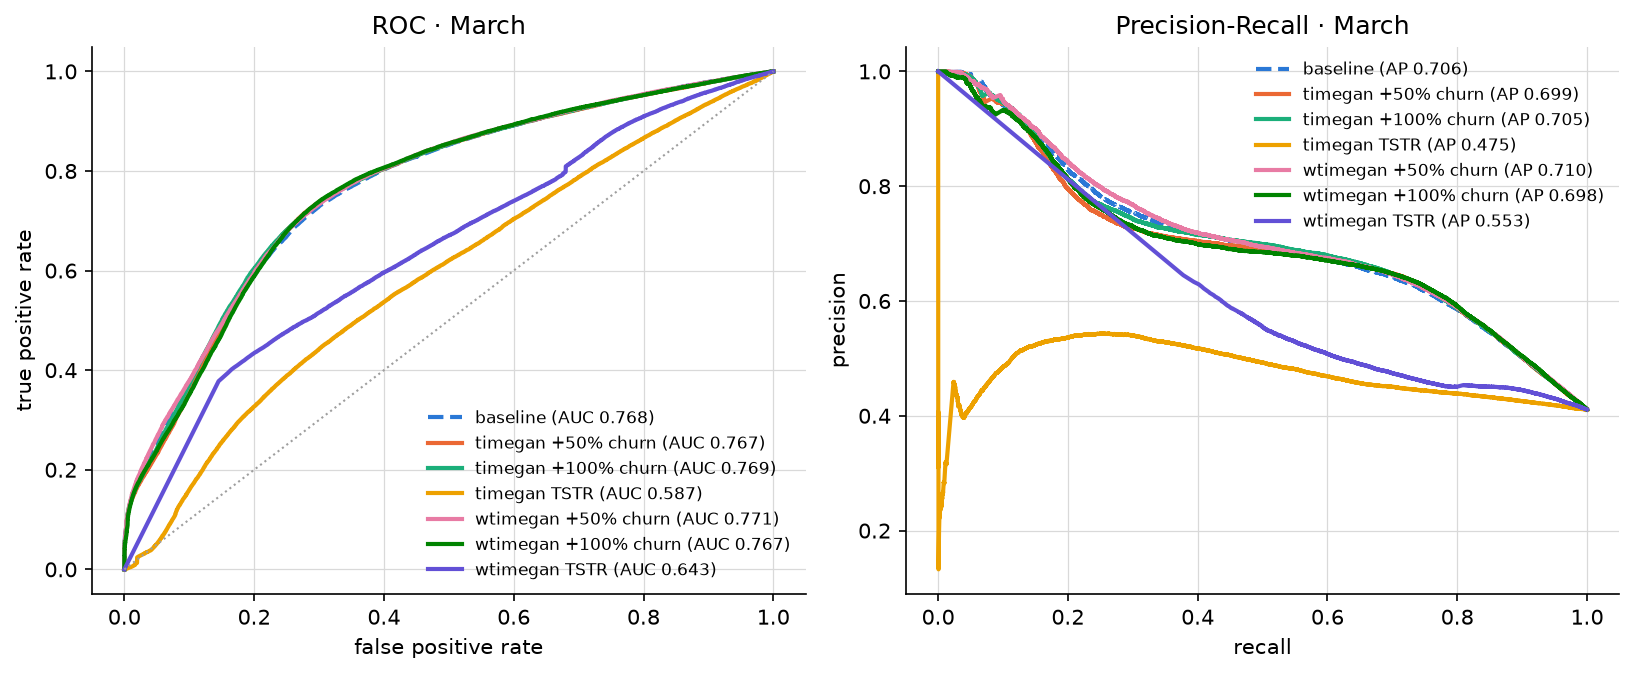
\includegraphics[width=0.49\textwidth]{figures/gan_models/bridge/roc_pr_lstm.png}
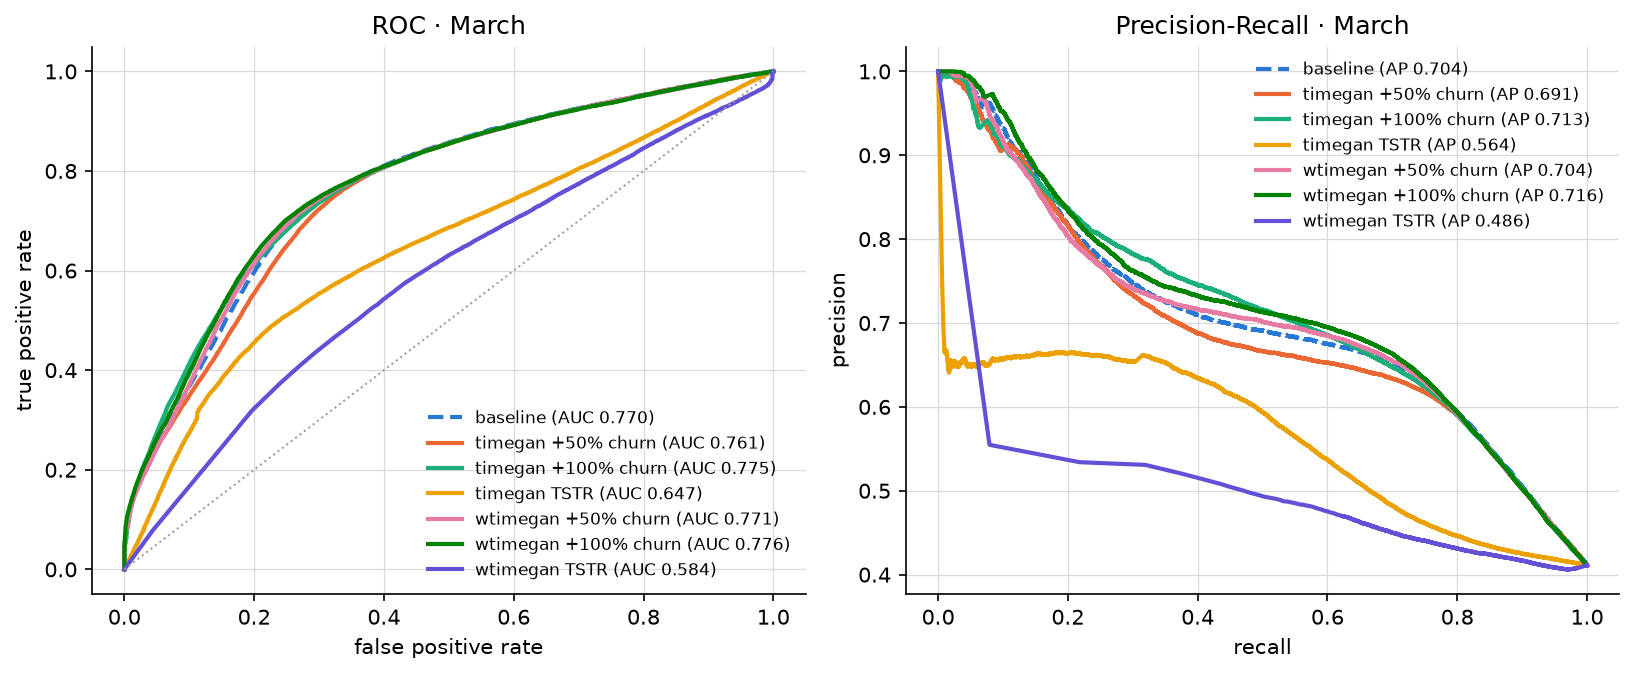
\includegraphics[width=0.49\textwidth]{figures/gan_models/bridge/roc_pr_gru.png}
\caption{ROC and precision-recall curves on March for the LSTM (left) and GRU (right) with TimeGAN and Wasserstein v1 customers. The augmented curves overlap the baseline; only the synthetic-only scenarios separate.}
\label{fig:w5_rocpr}
\end{figure}

\subsection{Behaviour Forecasters}

The forecasters of Workshop~2 read days 0 to 82 and predict days 83 to 89. They have no churn label: every synthetic customer brings its own input and its own target week, so the synthetic customers must reproduce the whole trajectory, payments included.

\begin{table}[H]
\centering
\renewcommand{\arraystretch}{1.3}
\begin{adjustbox}{max width=\textwidth}
\begin{tabular}{|l|l|rrrr|rrrr|}
\hline
 & & \multicolumn{4}{c|}{\textbf{LSTM}} & \multicolumn{4}{c|}{\textbf{GRU}} \\ \hline
\textbf{GAN} & \textbf{Scenario} & \textbf{MAE} & \textbf{Active} & \textbf{Pay} & \textbf{Week} & \textbf{MAE} & \textbf{Active} & \textbf{Pay} & \textbf{Week} \\ \hline
 & Baseline & 1.033 & 0.805 & 0.178 & 0.890 & 1.022 & 0.808 & 0.178 & 0.906 \\ \hline
\multirow{3}{*}{TimeGAN} & +50\% & 1.027 & 0.805 & 0.177 & 0.902 & 1.024 & 0.805 & 0.170 & 0.911 \\
 & +100\% & 1.019 & 0.806 & 0.175 & 0.900 & 1.029 & 0.802 & 0.168 & 0.904 \\
 & Synthetic only & 1.065 & 0.747 & 0.020 & 0.138 & 1.093 & 0.729 & 0.026 & 0.180 \\ \hline
\multirow{3}{*}{Wasserstein v1} & +50\% & 1.020 & 0.805 & 0.177 & 0.908 & 1.017 & 0.806 & 0.176 & 0.908 \\
 & +100\% & 1.024 & 0.804 & 0.170 & 0.899 & 1.021 & 0.801 & 0.173 & 0.908 \\
 & Synthetic only & 1.228 & 0.717 & 0.018 & 0.122 & 1.250 & 0.696 & 0.017 & 0.114 \\ \hline
\multirow{3}{*}{Wasserstein v2} & +50\% & 1.016 & 0.804 & 0.166 & 0.895 & 1.036 & 0.803 & 0.167 & 0.915 \\
 & +100\% & 1.028 & 0.804 & 0.174 & 0.901 & 1.022 & 0.803 & 0.167 & 0.901 \\
 & Synthetic only & \textbf{1.024} & \textbf{0.786} & \textbf{0.060} & \textbf{0.435} & \textbf{1.012} & \textbf{0.789} & \textbf{0.053} & \textbf{0.377} \\ \hline
\end{tabular}
\end{adjustbox}
\caption{Behaviour forecasters on real March customers. MAE: listening amounts (lower is better). Active: AUC of the daily \texttt{active} prediction. Pay: average precision of the daily payment prediction. Week: average precision of ``pays during the target week''. Bold: best synthetic-only result.}
\label{tab:w5_bridge_traj}
\end{table}

The augmented scenarios again stay within a few thousandths of the baseline. The synthetic-only scenario separates the parts of the trajectory that each GAN learned. A forecaster trained only on v2 customers predicts real March listening as well as one trained on real customers (MAE 1.024 against 1.033 for the LSTM, 1.012 against 1.022 for the GRU) and nearly matches the activity prediction (AUC 0.79 against 0.81), while TimeGAN and v1 customers clearly degrade both. Payments are where every GAN fails: the weekly payment average precision falls from 0.89 to 0.44 with v2 customers and to 0.14 with TimeGAN customers. This agrees with the payment checks of Section~\ref{sec:w5_domain}.

% ─────────────────────────────────────────────
\section{Conclusions}
% ─────────────────────────────────────────────

\paragraph{Vanilla GAN.} TimeGAN generates sequences in the right format, but its churners collapse to a few all-or-nothing patterns that the Workshop~2 classifier reads as exaggerated churners (churn probability 0.75 against 0.48). Its cross-entropy discriminator wins the game early, and the generator stops receiving a useful signal.

\paragraph{WGAN-GP.} The Wasserstein loss with gradient penalty gives a more stable game: the estimated distance stays low for the whole run, the generator keeps progressing, and the churner collapse disappears. Synthetic churners are as diverse as real ones and cover them, the Fréchet distance falls by a factor of 3.8 for churners and 3.2 for non-churners, and the churn probability of synthetic churners matches the real one. Applying WGAN-GP to TimeGAN required a change of critic: with a recurrent critic the gradient penalty runs without cuDNN and training was very inefficient; a temporal convolutional critic is 11 times faster per step and let us give the generator a full training budget in less time than the recurrent version.

\paragraph{What the GANs learn.} v2 reproduces listening and activity: a forecaster trained only on its customers predicts real listening as well as one trained on real data. It does not learn the renewal dynamics. Payments appear at a realistic rate but at days unrelated to the plan expiry, the expiry countdown does not follow its rule, synthetic non-churners are polarised, and a small classifier still separates real from synthetic customers about 90\,\% of the time.

\paragraph{Data augmentation.} Adding synthetic customers to the real training data does not improve the Workshop~2 classifiers or forecasters; the changes are of the size of training noise. The synthetic-only experiment shows how much of the real signal each GAN captured, and v2 captures the most.

\paragraph{Limitations.} The main configuration was fixed to the published defaults, with only the generator learning rate and the joint-phase length of v2 set from a pilot run. The later search used a reduced budget, and for the non-churners its configurations did worse at full budget than the hand-set one; that hand-set configuration was run with a single seed, so the comparison between the two is not confirmed. The ranking of v2 above TimeGAN does hold over five seeds (Section~\ref{sec:w5_robustness}). The quality analysis and each augmentation scenario use one seed, so the augmentation differences are not separated from training noise. TimeGAN is unconditional, so one model is trained per class and the class balance of the synthetic data is set by hand. v2 changes both the adversarial loss and the critic architecture with respect to TimeGAN, so its gain cannot be attributed to the Wasserstein loss alone. The Fréchet distance uses the Workshop~2 LSTM as feature extractor and measures realism only as that model sees it. A natural next step is to keep the GAN for listening and activity and to generate payments with the renewal rules (pay near the expiry, rebuild the state), which is the part no GAN learned.

\begin{thebibliography}{99}

\bibitem{arjovsky2017}
Arjovsky, M., Chintala, S., \& Bottou, L. (2017).
\textit{Wasserstein generative adversarial networks}.
In Proceedings of the 34th International Conference on Machine Learning (ICML), 214--223. arXiv:1701.07875.

\bibitem{bai2018}
Bai, S., Kolter, J. Z., \& Koltun, V. (2018).
\textit{An empirical evaluation of generic convolutional and recurrent networks for sequence modeling}.
arXiv:1803.01271. \url{https://arxiv.org/abs/1803.01271}

\bibitem{donahue2019}
Donahue, C., McAuley, J., \& Puckette, M. (2019).
\textit{Adversarial audio synthesis}.
In International Conference on Learning Representations (ICLR). arXiv:1802.04208.

\bibitem{goodfellow2014}
Goodfellow, I., Pouget-Abadie, J., Mirza, M., Xu, B., Warde-Farley, D., Ozair, S., Courville, A., \& Bengio, Y. (2014).
\textit{Generative adversarial nets}.
In Advances in Neural Information Processing Systems 27 (NeurIPS). arXiv:1406.2661.

\bibitem{gulrajani2017}
Gulrajani, I., Ahmed, F., Arjovsky, M., Dumoulin, V., \& Courville, A. (2017).
\textit{Improved training of Wasserstein GANs}.
In Advances in Neural Information Processing Systems 30 (NeurIPS). arXiv:1704.00028.

\bibitem{heusel2017}
Heusel, M., Ramsauer, H., Unterthiner, T., Nessler, B., \& Hochreiter, S. (2017).
\textit{GANs trained by a two time-scale update rule converge to a local Nash equilibrium}.
In Advances in Neural Information Processing Systems 30 (NeurIPS). arXiv:1706.08500.

\bibitem{kkbox2017}
KKBOX. (2017).
\textit{WSDM--KKBox's Churn Prediction Challenge} [Data set and competition].
Kaggle. \url{https://www.kaggle.com/competitions/kkbox-churn-prediction-challenge}

\bibitem{wiese2020}
Wiese, M., Knobloch, R., Korn, R., \& Kretschmer, P. (2020).
\textit{Quant GANs: Deep generation of financial time series}.
Quantitative Finance, 20(9), 1419--1440. arXiv:1907.06673.

\bibitem{yoon2019}
Yoon, J., Jarrett, D., \& van der Schaar, M. (2019).
\textit{Time-series generative adversarial networks}.
In Advances in Neural Information Processing Systems 32 (NeurIPS).

\bibitem{zhu2019}
Zhu, F., Ye, F., Fu, Y., Liu, Q., \& Shen, B. (2019).
\textit{Electrocardiogram generation with a bidirectional LSTM-CNN generative adversarial network}.
Scientific Reports, 9, 6734. \url{https://doi.org/10.1038/s41598-019-42516-z}

\end{thebibliography}

\end{document}
